%–––––––––––––––––––––––––––––––––––––––––––––––
% main.tex
% Master file that pulls everything together
%–––––––––––––––––––––––––––––––––––––––––––––––

\documentclass[10pt]{beamer}

% load your custom preamble
% Beamer theme
\usetheme{moloch}
\molochset{
  progressbar=frametitle
}

\setbeamertemplate{page number in head/foot}[framenumber]

\usepackage{lmodern}
\usefonttheme{professionalfonts}   % don’t override your chosen fonts
\usefonttheme[onlymath]{serif}     % use a serif font just for math


\usepackage{appendixnumberbeamer}

% Common packages
\usepackage{booktabs}
\usepackage[scale=2]{ccicons}
\usepackage{pgfplots}
\usepgfplotslibrary{dateplot}
\usepackage{xspace}

% Custom macros
\newcommand{\themename}{\textbf{\textsc{metropolis}}\xspace}


\usepackage{amsmath}   % for \operatornamewithlimits, \argmin, etc.
\usepackage{amssymb}   % for \mathbb (and loads amsfonts)
\usepackage{bm}
\usepackage[x11names,svgnames,table]{xcolor}

\definecolor{orange}{HTML}{eb811b}
\definecolor{green}{HTML}{008080}



\usepackage{array}      % For extended column formatting
\usepackage{caption}    % For customizing captions
\usepackage{subcaption} % provides the subfigure environment


\usepackage{graphicx}    % \includegraphics
\usepackage{tikz}
\usetikzlibrary{spy,shapes.misc}
\usepackage{calc}
\usepackage{multirow}



% bibliography
% \usepackage[style=authoryear,backend=biber,maxnames=99,giveninits=true]{biblatex}


\usepackage[
  backend=biber,            % use Biber
  style=authoryear,         % author–year style as a basis
  maxcitenames=1,           % when >1 author, show “<First> et al.”
  mincitenames=1,           % same for the first citation
  uniquelist=false          % don’t force extra names to disambiguate
]{biblatex}

\addbibresource{biblio/references.bib} 

\renewcommand*{\mkbibparens}[1]{\mkbibbrackets{#1}}

% if you prefer \cite rather than \parencite:
\let\cite\parencite



\setbeamerfont{bibliography item}{size=\scriptsize}
\setbeamerfont{bibliography entry author}{size=\scriptsize}
\setbeamerfont{bibliography entry title}{size=\scriptsize}
\setbeamerfont{bibliography entry location}{size=\scriptsize}
\setbeamerfont{bibliography entry note}{size=\scriptsize}
\newcommand{\bolda}{\bm{a}}
\newcommand{\boldb}{\bm{b}}
\newcommand{\boldc}{\bm{c}}
\newcommand{\boldd}{\bm{d}}
\newcommand{\bolde}{\bm{e}}
\newcommand{\boldf}{\bm{f}}
\newcommand{\boldg}{\bm{g}}
\newcommand{\boldh}{\bm{h}}
\newcommand{\boldi}{\bm{i}}
\newcommand{\boldj}{\bm{j}}
\newcommand{\boldk}{\bm{k}}
\newcommand{\boldl}{\bm{l}}
\newcommand{\boldm}{\bm{m}}
\newcommand{\boldn}{\bm{n}}
\newcommand{\boldo}{\bm{o}}
\newcommand{\boldp}{\bm{p}}
\newcommand{\boldq}{\bm{q}}
\newcommand{\boldr}{\bm{r}}
\newcommand{\bolds}{\bm{s}}
\newcommand{\boldt}{\bm{t}}
\newcommand{\boldu}{\bm{u}}
\newcommand{\boldv}{\bm{v}}
\newcommand{\boldw}{\bm{w}}
\newcommand{\boldx}{\bm{x}}
\newcommand{\boldy}{\bm{y}}
\newcommand{\boldz}{\bm{z}}

\newcommand{\boldmu}{\bm{\mu}}
\newcommand{\boldxi}{\bm{\xi}}
\newcommand{\bbR}{\mathbb{R}}
\newcommand{\boldlambda}{\bm{\lambda}}
\newcommand{\lambdahat}{\hat{\lambda}}
\newcommand{\boldlambdahat}{\bm{\hat{\lambda}}}
\newcommand{\boldgbar}{\bar{\boldg}}
\newcommand{\boldpbar}{\bar{\boldp}}

\newcommand{\boldA}{\bm{A}}
\newcommand{\boldB}{\bm{B}}
\newcommand{\boldC}{\bm{C}}
\newcommand{\boldD}{\bm{D}}
\newcommand{\boldE}{\bm{E}}
\newcommand{\boldF}{\bm{F}}
\newcommand{\boldG}{\bm{G}}
\newcommand{\boldH}{\bm{H}}
\newcommand{\boldI}{\bm{I}}
\newcommand{\boldJ}{\bm{J}}
\newcommand{\boldK}{\bm{K}}
\newcommand{\boldL}{\bm{L}}
\newcommand{\boldM}{\bm{M}}
\newcommand{\boldN}{\bm{N}}
\newcommand{\boldO}{\bm{O}}
\newcommand{\boldP}{\bm{P}}
\newcommand{\boldQ}{\bm{Q}}
\newcommand{\boldR}{\bm{R}}
\newcommand{\boldS}{\bm{S}}
\newcommand{\boldT}{\bm{T}}
\newcommand{\boldU}{\bm{U}}
\newcommand{\boldV}{\bm{V}}
\newcommand{\boldW}{\bm{W}}
\newcommand{\boldX}{\bm{X}}
\newcommand{\boldY}{\bm{Y}}
\newcommand{\boldZ}{\bm{Z}}







\newcommand{\calA}{\mathcal{A}}
\newcommand{\calB}{\mathcal{B}}
\newcommand{\calC}{\mathcal{C}}
\newcommand{\calD}{\mathcal{D}}
\newcommand{\calE}{\mathcal{E}}
\newcommand{\calF}{\mathcal{F}}
\newcommand{\calG}{\mathcal{G}}
\newcommand{\calH}{\mathcal{H}}
\newcommand{\calI}{\mathcal{I}}
\newcommand{\calJ}{\mathcal{J}}
\newcommand{\calK}{\mathcal{K}}
\newcommand{\calL}{\mathcal{L}}
\newcommand{\calM}{\mathcal{M}}
\newcommand{\calN}{\mathcal{N}}
\newcommand{\calO}{\mathcal{O}}
\newcommand{\calP}{\mathcal{P}}
\newcommand{\calQ}{\mathcal{Q}}
\newcommand{\calR}{\mathcal{R}}
\newcommand{\calS}{\mathcal{S}}
\newcommand{\calT}{\mathcal{T}}
\newcommand{\calU}{\mathcal{U}}
\newcommand{\calV}{\mathcal{V}}
\newcommand{\calW}{\mathcal{W}}
\newcommand{\calX}{\mathcal{X}}
\newcommand{\calY}{\mathcal{Y}}
\newcommand{\calZ}{\mathcal{Z}}


\newcommand{\boldcalT}{\bm{\calT}}
\newcommand{\boldcalW}{\bm{\calW}}
\newcommand{\boldcalA}{\bm{\calA}}
\newcommand{\boldcalR}{\bm{\calR}}


\newcommand{\rma}{\mathrm{a}}
\newcommand{\rmb}{\mathrm{b}}
\newcommand{\rmc}{\mathrm{c}}
\newcommand{\rmd}{\mathrm{d}}
\newcommand{\rme}{\mathrm{e}}
\newcommand{\rmf}{\mathrm{f}}
\newcommand{\rmg}{\mathrm{g}}
\newcommand{\rmh}{\mathrm{h}}
\newcommand{\rmi}{\mathrm{i}}
\newcommand{\rmj}{\mathrm{j}}
\newcommand{\rmk}{\mathrm{k}}
\newcommand{\rml}{\mathrm{l}}
\newcommand{\rmm}{\mathrm{m}}
\newcommand{\rmn}{\mathrm{n}}
\newcommand{\rmo}{\mathrm{o}}
\newcommand{\rmp}{\mathrm{p}}
\newcommand{\rmq}{\mathrm{q}}
\newcommand{\rmr}{\mathrm{r}}
\newcommand{\rms}{\mathrm{s}}
\newcommand{\rmt}{\mathrm{t}}
\newcommand{\rmu}{\mathrm{u}}
\newcommand{\rmv}{\mathrm{v}}
\newcommand{\rmw}{\mathrm{w}}
\newcommand{\rmx}{\mathrm{x}}
\newcommand{\rmy}{\mathrm{y}}
\newcommand{\rmz}{\mathrm{z}}

\newcommand{\rmA}{\mathrm{A}}
\newcommand{\rmB}{\mathrm{B}}
\newcommand{\rmC}{\mathrm{C}}
\newcommand{\rmD}{\mathrm{D}}
\newcommand{\rmE}{\mathrm{E}}
\newcommand{\rmF}{\mathrm{F}}
\newcommand{\rmG}{\mathrm{G}}
\newcommand{\rmH}{\mathrm{H}}
\newcommand{\rmI}{\mathrm{I}}
\newcommand{\rmJ}{\mathrm{J}}
\newcommand{\rmK}{\mathrm{K}}
\newcommand{\rmL}{\mathrm{L}}
\newcommand{\rmM}{\mathrm{M}}
\newcommand{\rmN}{\mathrm{N}}
\newcommand{\rmO}{\mathrm{O}}
\newcommand{\rmP}{\mathrm{P}}
\newcommand{\rmQ}{\mathrm{Q}}
\newcommand{\rmR}{\mathrm{R}}
\newcommand{\rmS}{\mathrm{S}}
\newcommand{\rmT}{\mathrm{T}}
\newcommand{\rmU}{\mathrm{U}}
\newcommand{\rmV}{\mathrm{V}}
\newcommand{\rmW}{\mathrm{W}}
\newcommand{\rmX}{\mathrm{X}}
\newcommand{\rmY}{\mathrm{Y}}
\newcommand{\rmZ}{\mathrm{Z}}


\newcommand{\boldSigma}{\bm{\Sigma}}

\newcommand{\boldzero}{\bm{0}}
\newcommand{\boldphi}{\bm{\phi}}
\newcommand{\R}{\mathbb{R}}


\newcommand{\transp}{^\top}
\newcommand{\argmin}{\operatornamewithlimits{arg\,min}}




\definecolor{mDarkTeal}{HTML}{23373b}




% Presentation metadata
\title{Solving Blind Inverse Problems:\\ Adaptive Diffusion Models for Motion-Corrected Sparse-View 4DCT}
% \subtitle{A modern beamer theme}
\author[De Paepe \and Bousse \and Phung-Ngoc \and Visvikis]{%
  \underline{Antoine De Paepe}\inst{1}
  \and
  Alexandre Bousse\inst{1}
  \and
  Cl{\'e}mentine Phung-Ngoc\inst{1}
  \and
  Dimitris Visvikis\inst{1}
}\institute{\inst{1} University of Western Brittany, LaTIM, UMR Inserm 1101, 29238 Brest, France}


\date{Fully 3D 2025, Shanghai, China - May 27, 2025}

% end local group (bg resets here)


% graphics path
\graphicspath{{figures/}}
\usetikzlibrary{positioning}

\begin{document}

  {
  \setbeamercolor{background canvas}{bg=mDarkTeal}
  \setbeamercolor{normal text}{fg=white}
    \begin{frame}
      \maketitle
      \begin{tikzpicture}[overlay, remember picture]
      \node[above =1cm of current page.south, xshift=2cm, yshift=-0.5cm] {
\includegraphics[width=6cm]{figures/cover/logo.png}};
      \end{tikzpicture}
    \end{frame}
  }


  % include each content file in order
  %–––––––––––––––––––––––––––––––––––––––––––––––
% content/01_introduction.tex
%–––––––––––––––––––––––––––––––––––––––––––––––

\section{Introduction}


\begin{frame}[t, fragile]
  \frametitle{Introduction to Lung CT}

  \begin{itemize}
    \item<1-> \textbf{Lung CT Reconstruction}: The reconstruction of lung CT images can be formulated as the following optimization problem:
          \begin{equation*}
            \min_{\textcolor{green}{\boldx}} \frac{1}{2}\left\| \boldcalR \textcolor{green}{\boldx} - \boldb \right\|_{W}^2 + \boldR(\textcolor{green}{\boldx})
          \end{equation*}
    \item<2-> \textbf{Limitations of Static CT}:
          \begin{itemize}
            \item Assumes the patient remains stationary during the scan.
            \item Respiratory motion can introduce artifacts and blurring.
          \end{itemize}
    \item<3-> \textbf{Introduction to 4DCT}:
          \begin{itemize}
            \item Captures 3D images across respiratory phases, enabling dynamic lung motion visualization.
            \item Essential for applications like radiotherapy planning \cite{kwong2015f}.
          \end{itemize}
  \end{itemize}
\end{frame}

\begin{frame}[t, fragile]

  \frametitle{Introduction to Dynamic Lung CT}

  \begin{itemize}
    \item<1-> \textbf{4DCT Acquisition Modes}:
          \begin{itemize}
            \item Helical mode: The scanner rotates continuously as the patient table moves through the gantry.
            \item Cine mode: The scanner acquires multiple images at the same table position over a period.
            \item Uses a surrogate signal (e.g., respiratory belt or external marker) to track breathing motion.
          \end{itemize}
    \item<2-> \textbf{Example of Helical 4DCT Acquisition}:

  \end{itemize}

  \only<3>{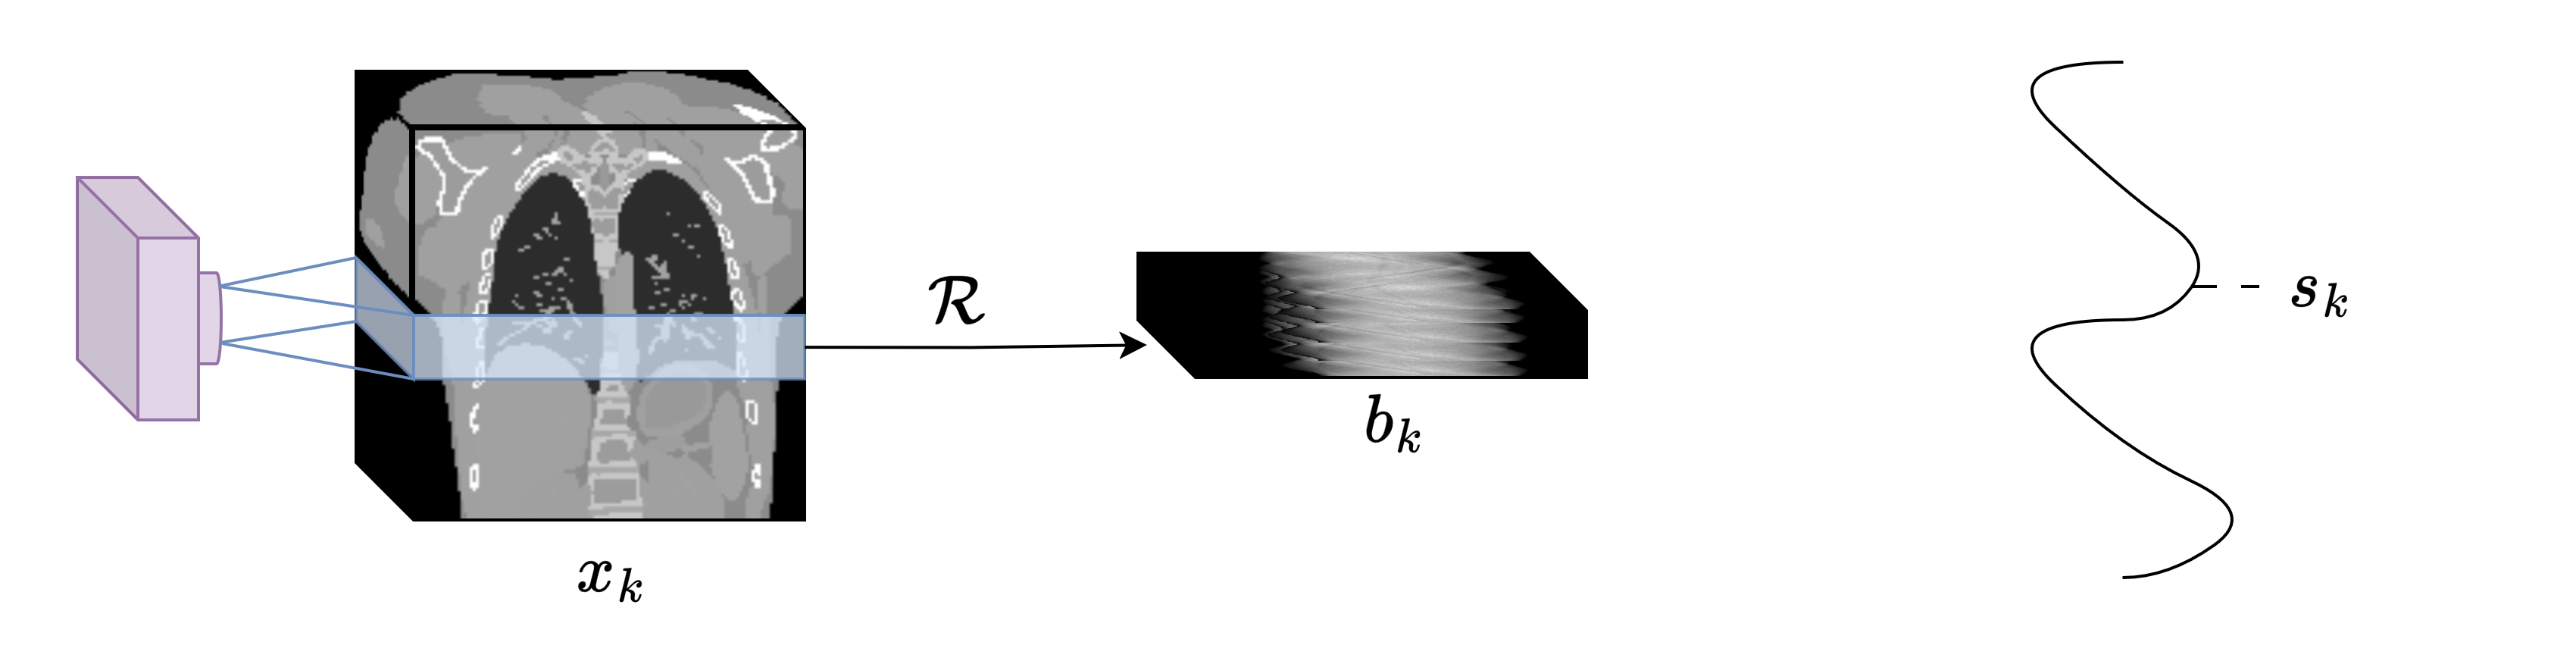
\includegraphics[width=1\linewidth]{figures/intro/acquisition/acqu1.png}}
  \only<4>{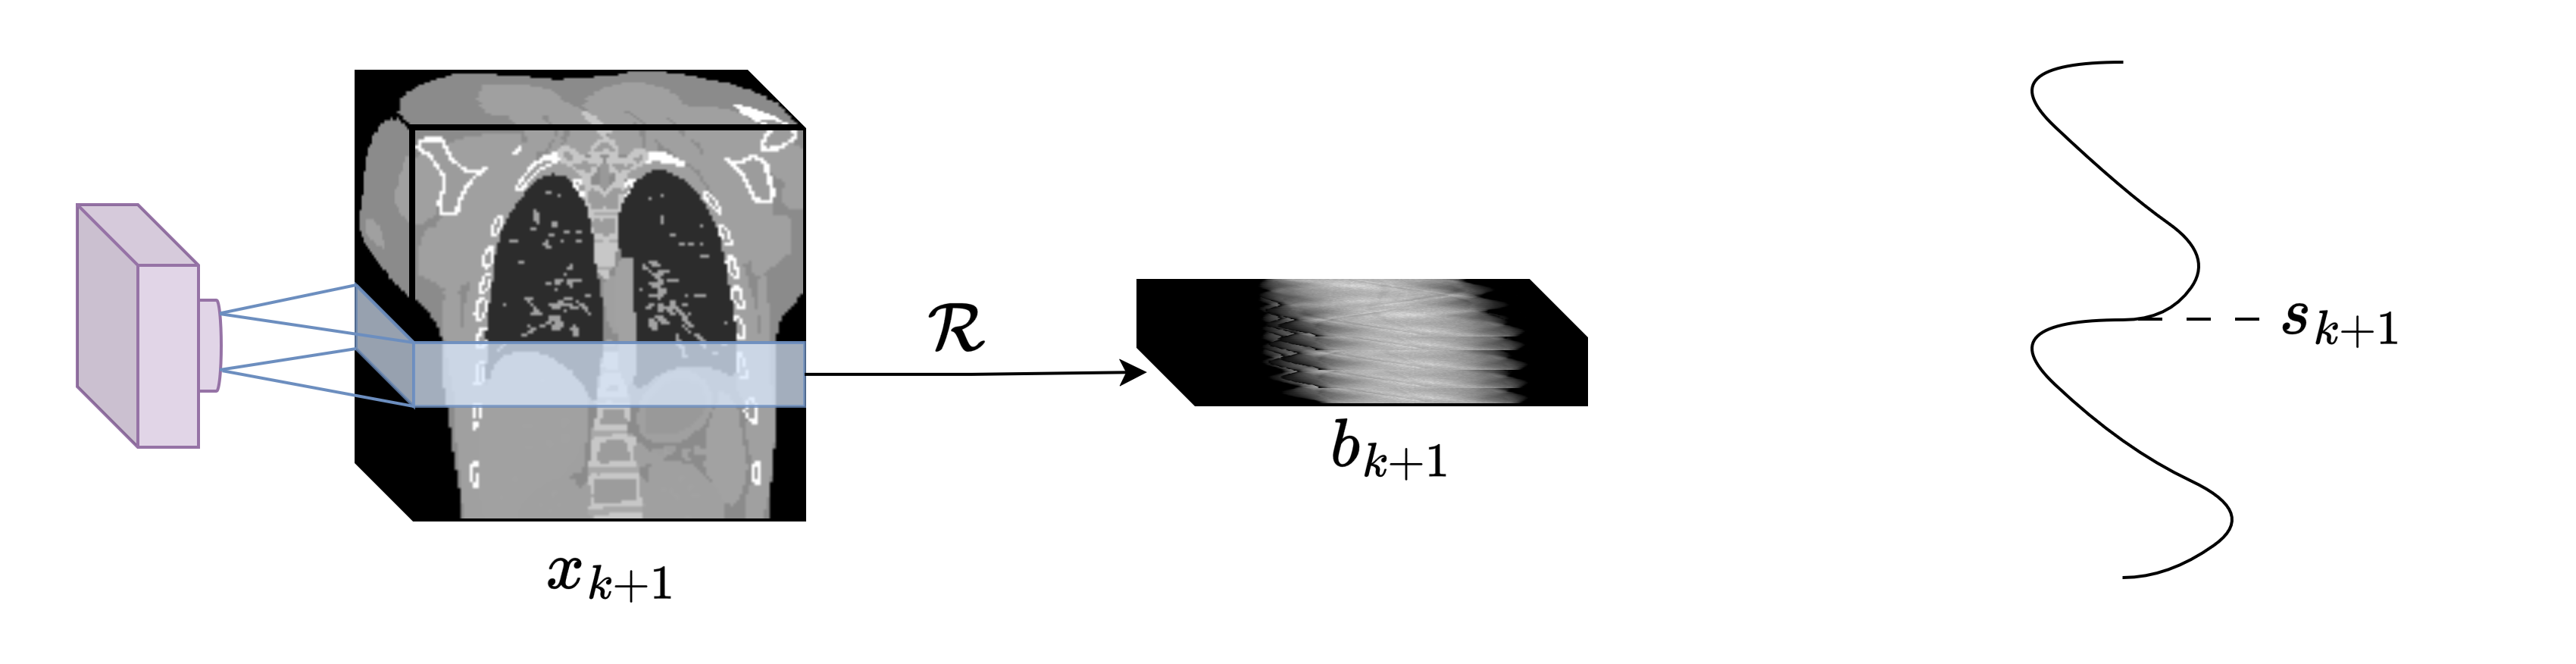
\includegraphics[width=1\linewidth]{figures/intro/acquisition/acqu2.png}}
  \only<5>{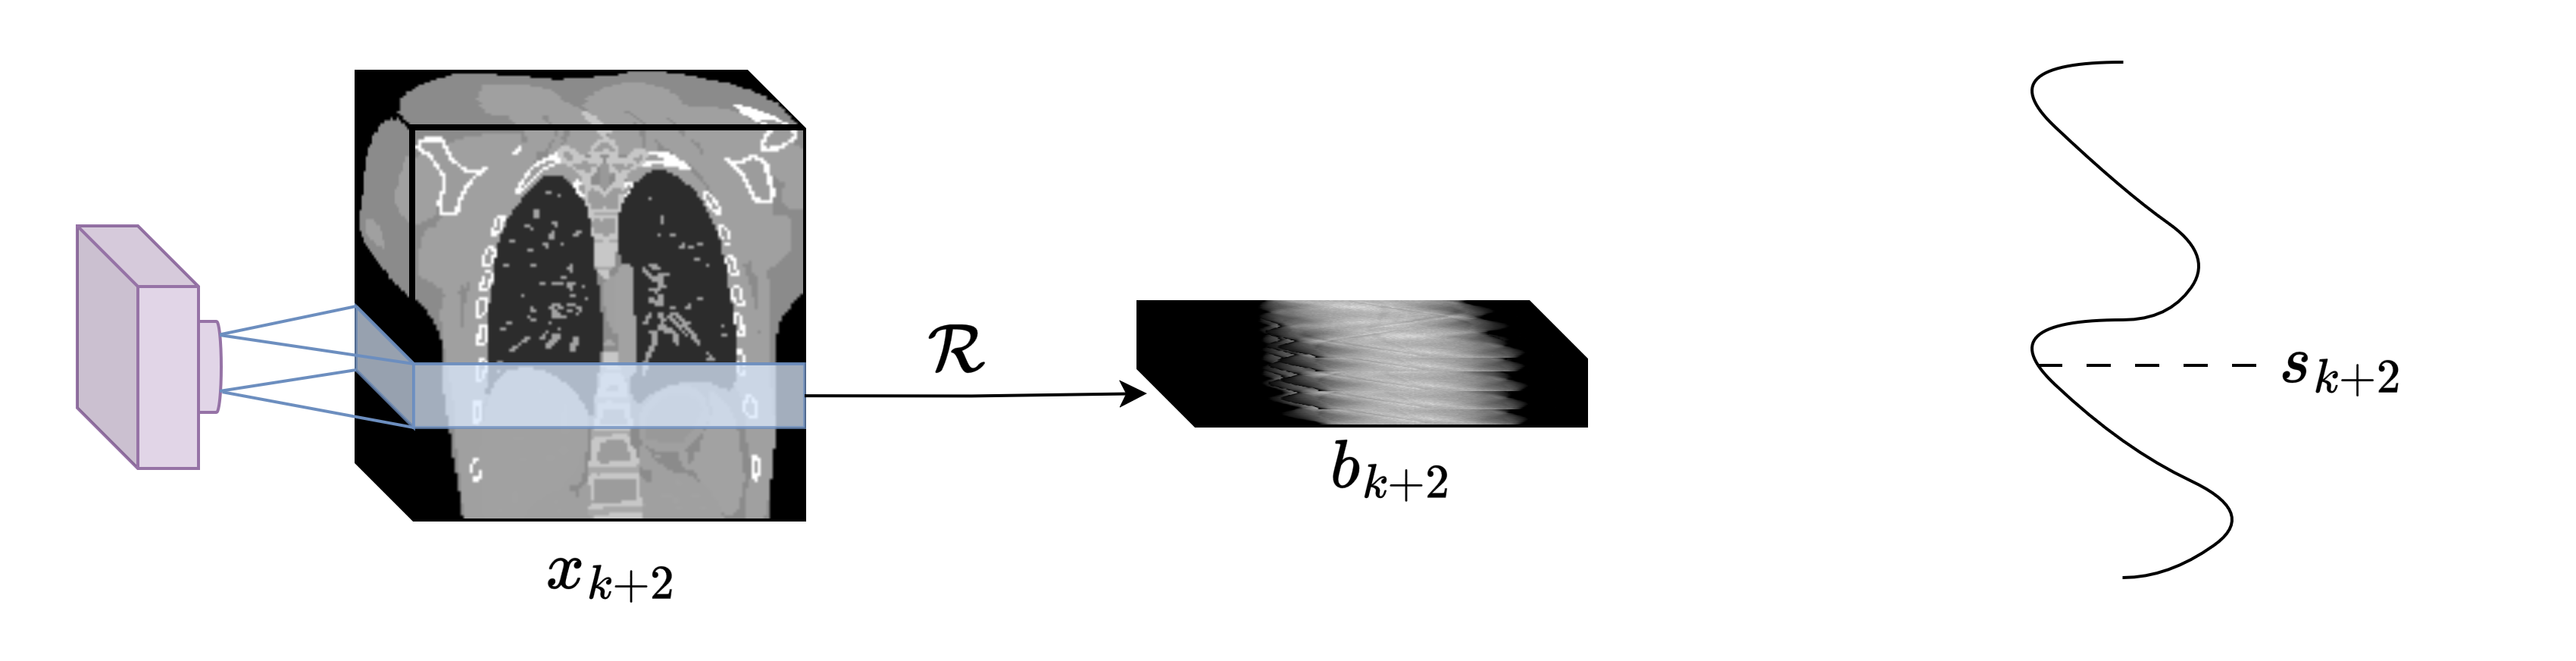
\includegraphics[width=1\linewidth]{figures/intro/acquisition/acqu3.png}}
  \only<6>{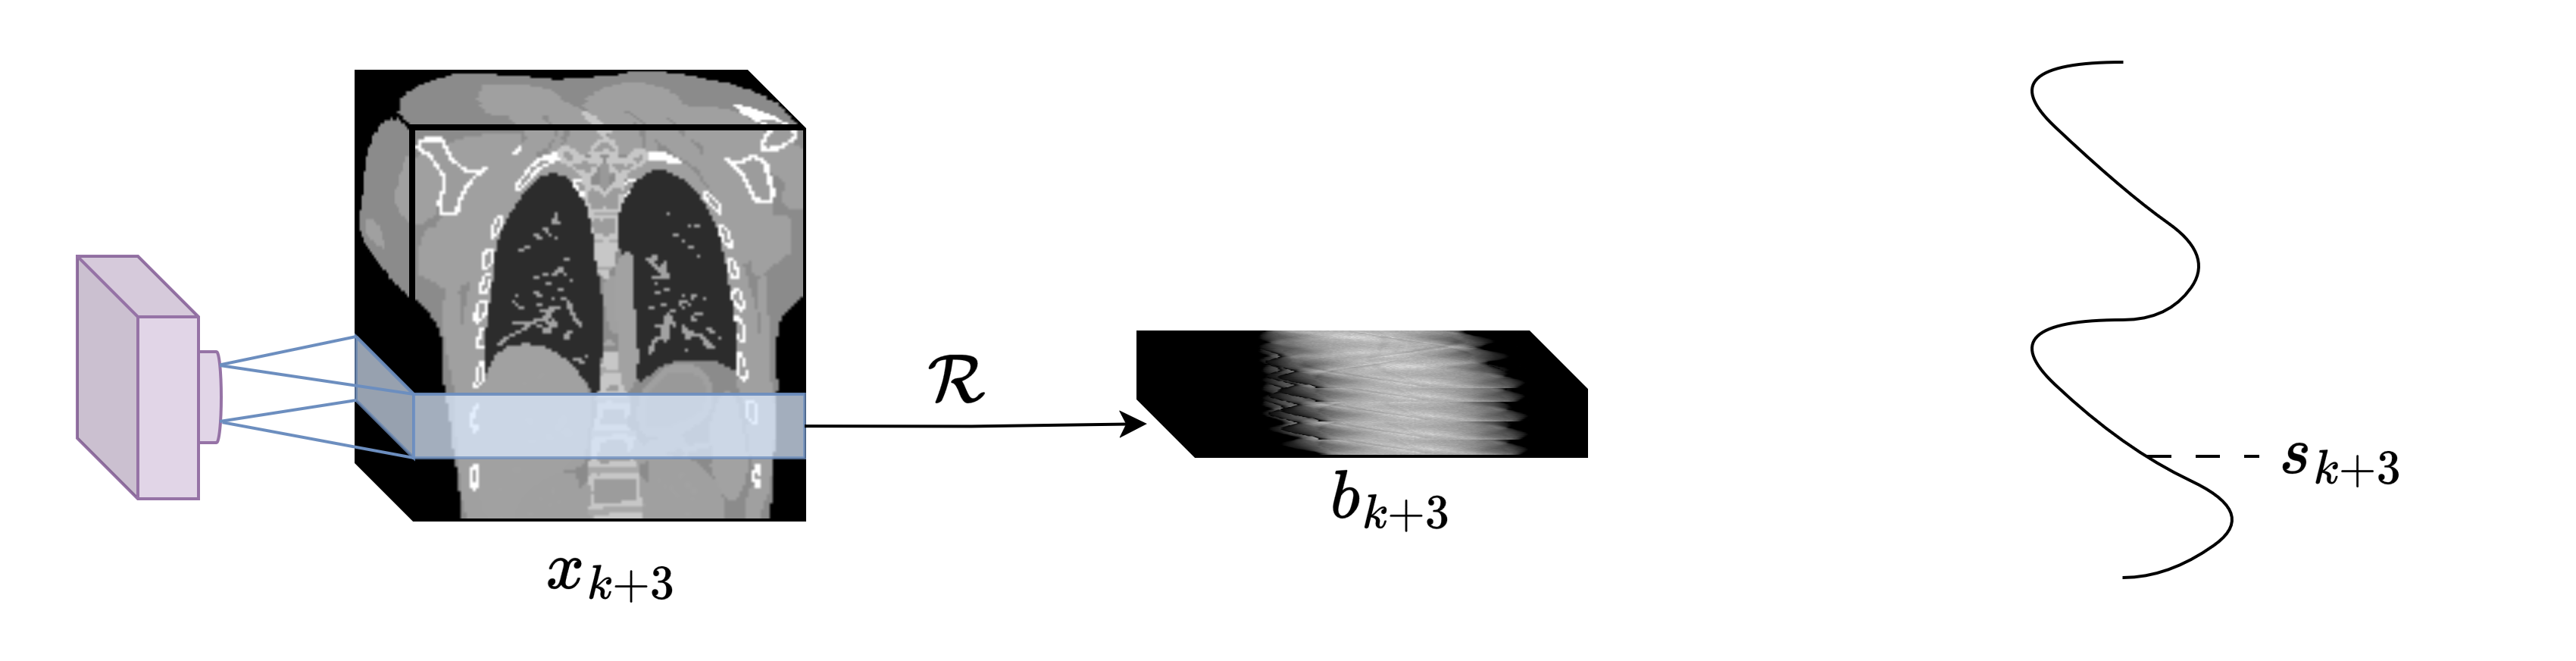
\includegraphics[width=1\linewidth]{figures/intro/acquisition/acqu4.png}}

\end{frame}



\begin{frame}[t, fragile]
  \frametitle{Challenges in 4DCT}

  % Show first two images only on specific overlays
  \only<1>{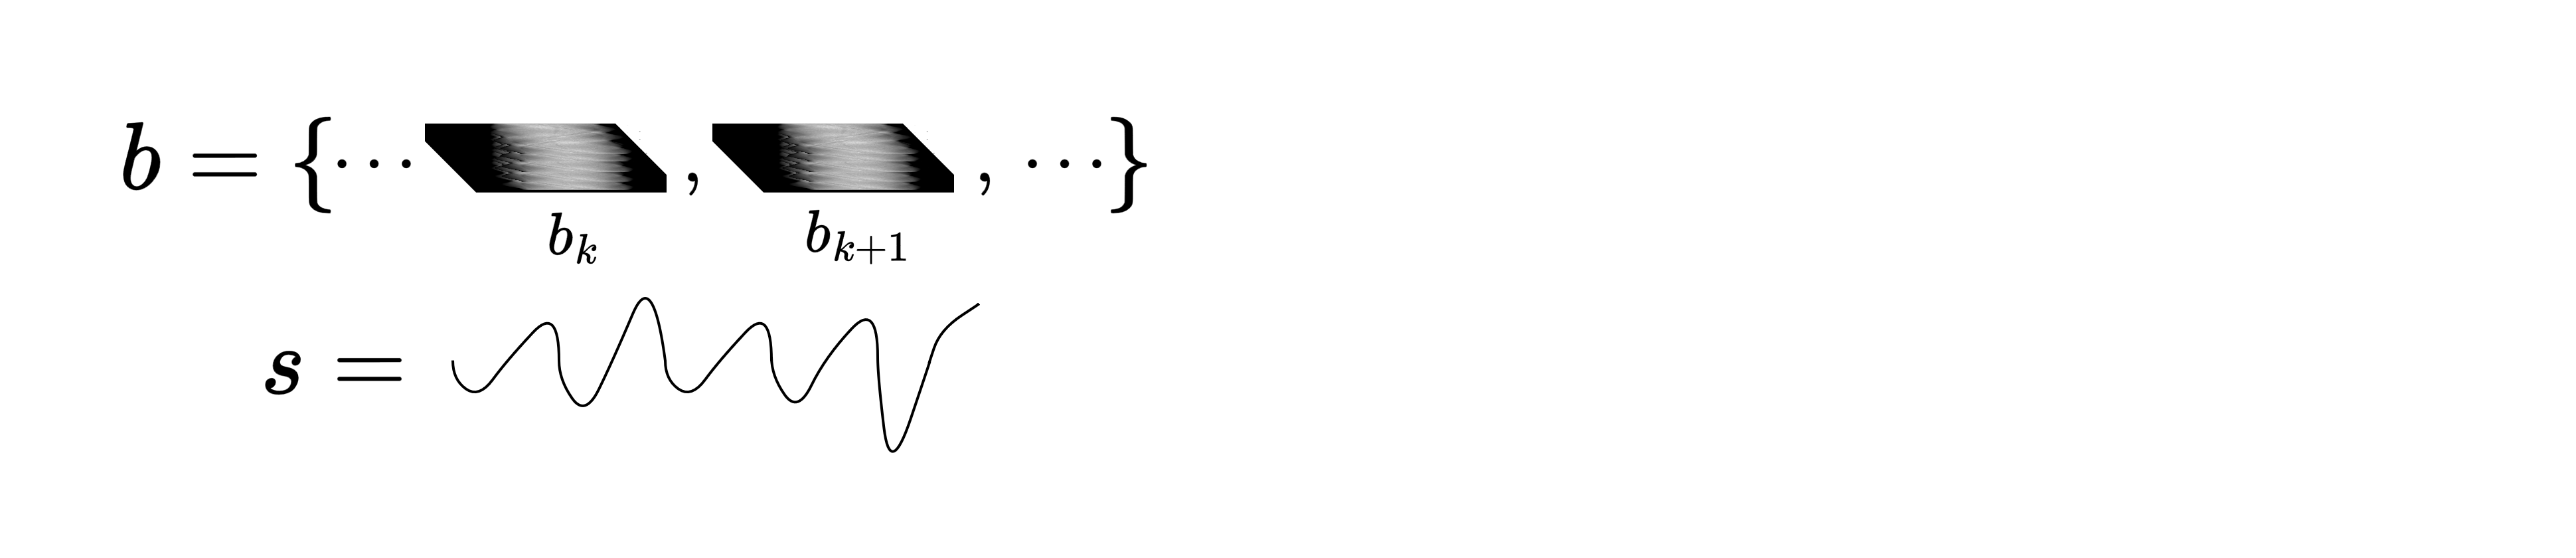
\includegraphics[width=1\linewidth]{figures/intro/gating_reco/gating1.png}}
  \only<2>{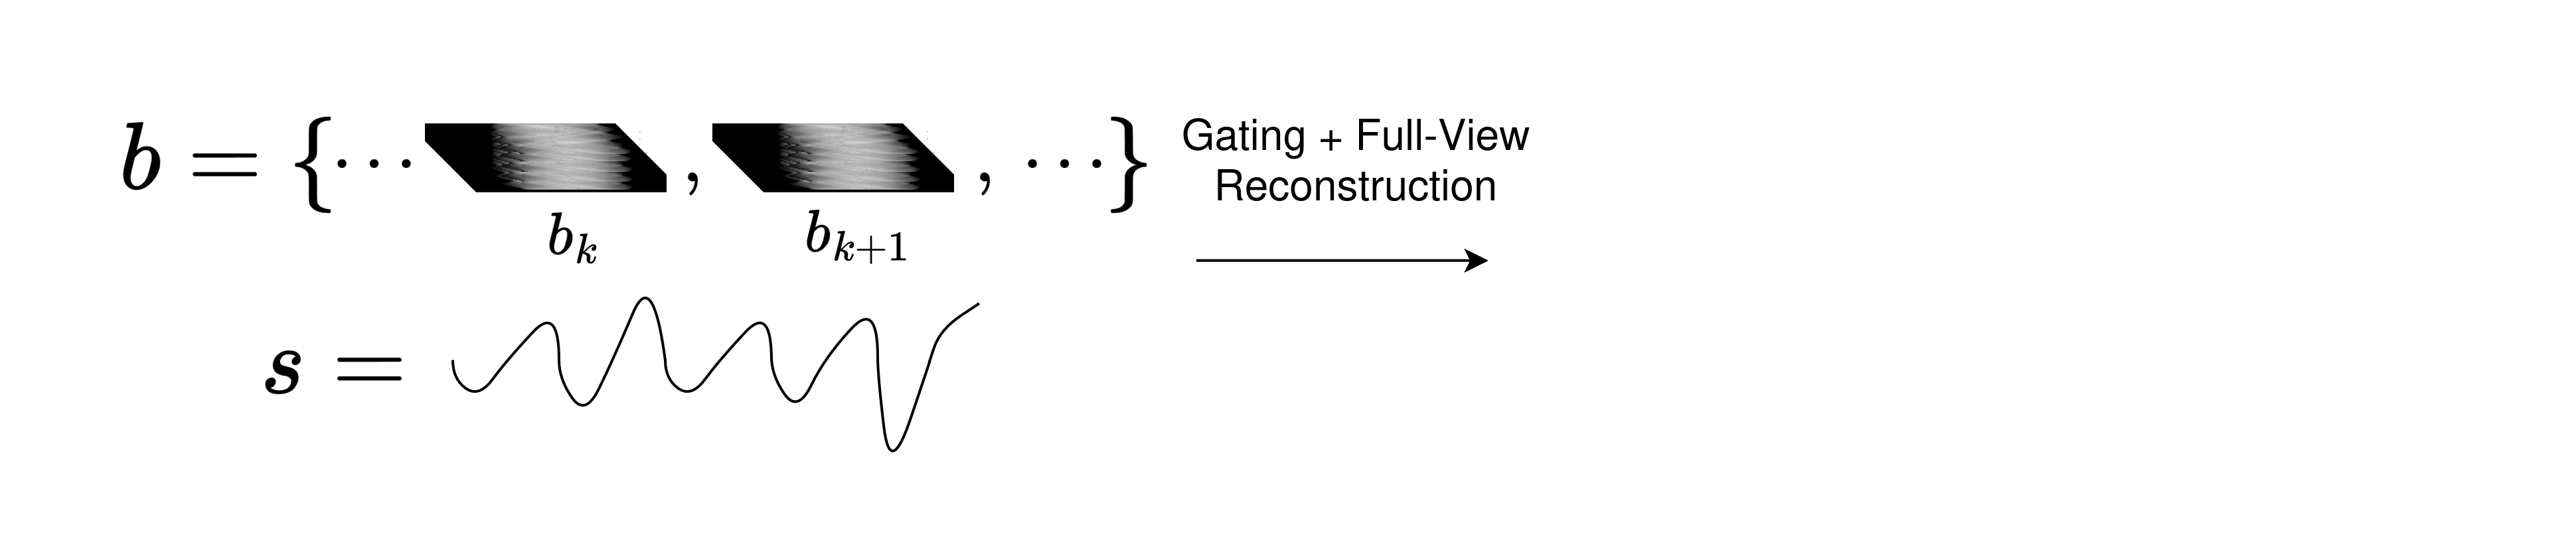
\includegraphics[width=1\linewidth]{figures/intro/gating_reco/gating2.png}}

  % Keep third image from slide 3 onwards
  \only<3->{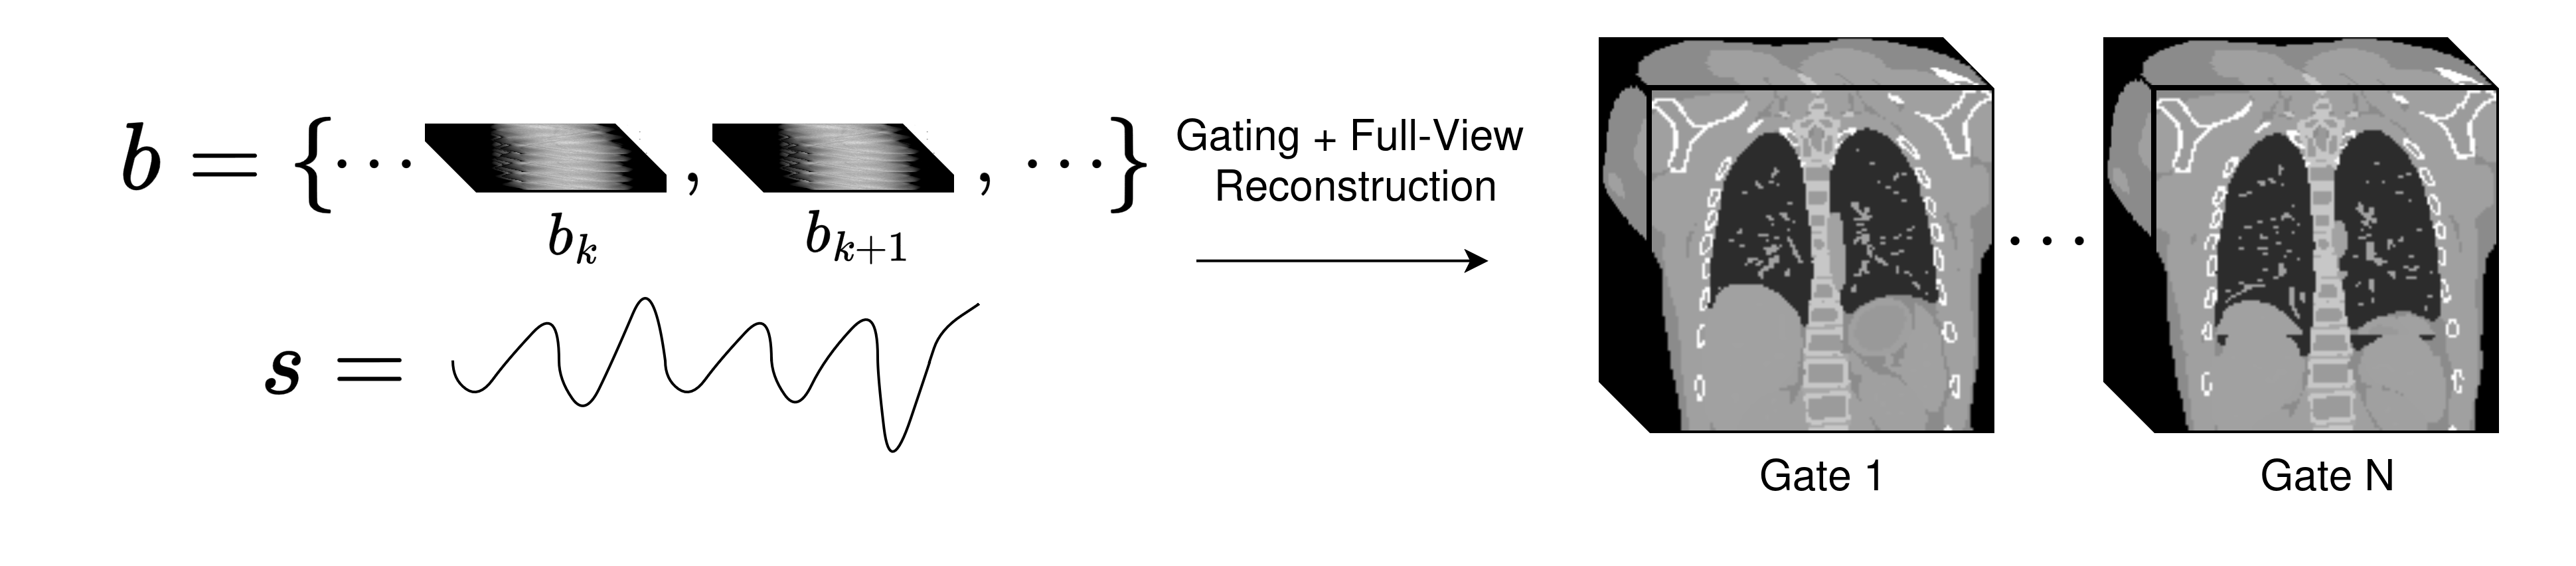
\includegraphics[width=1\linewidth]{figures/intro/gating_reco/gating3.png}}

  \vspace{0.3cm}

  \only<4->{
    \begin{itemize}
      \item<4-> \textbf{Challenges:}
            \begin{itemize}
              \item Motion artifacts due to irregular breathing patterns.
              \item Surrogate signals may not always be stored.
              \item Increased radiation dose from multiple phase acquisitions; necessitates dose reduction strategies.
            \end{itemize}
    \end{itemize}
  }
\end{frame}


\begin{frame}[t, fragile]
\frametitle{Joint Reconstruction \& Motion Estimation (JRM)}

    \begin{itemize}
    \item<1-> \textbf{General JRM Framework:}
              \begin{equation*}
              \min_{\textcolor{green}{\boldx},  \textcolor{orange}{\bold{\varphi}}} \frac{1}{2}\left\| \boldcalA_{\textcolor{orange}{\bold{\varphi}}} \textcolor{green}{\boldx} - \boldb \right\|_{W}^2 + \boldR(\textcolor{green}{\boldx})
            \end{equation*}

            where $\textcolor{orange}{\bold{\varphi}}$ are motion parameters.

      \item<2-> \textbf{4DCT JRM Framework \cite{huang2024resolving}:}
            \begin{equation*}
              \min_{\textcolor{green}{\boldx},  \textcolor{orange}{\boldphi}, \textcolor{orange}{\bolds}} \frac{1}{2}\sum_{k = 1}^{n_t}\left\| \boldcalR \circ \boldcalT_{k} \circ \boldcalW_{\textcolor{orange}{\boldphi} \cdot \textcolor{orange}{\bolds_k} } \textcolor{green}{\boldx} - \boldb_k \right\|_{W}^2 + \boldR(\textcolor{green}{\boldx})
            \end{equation*}

            \only<3>{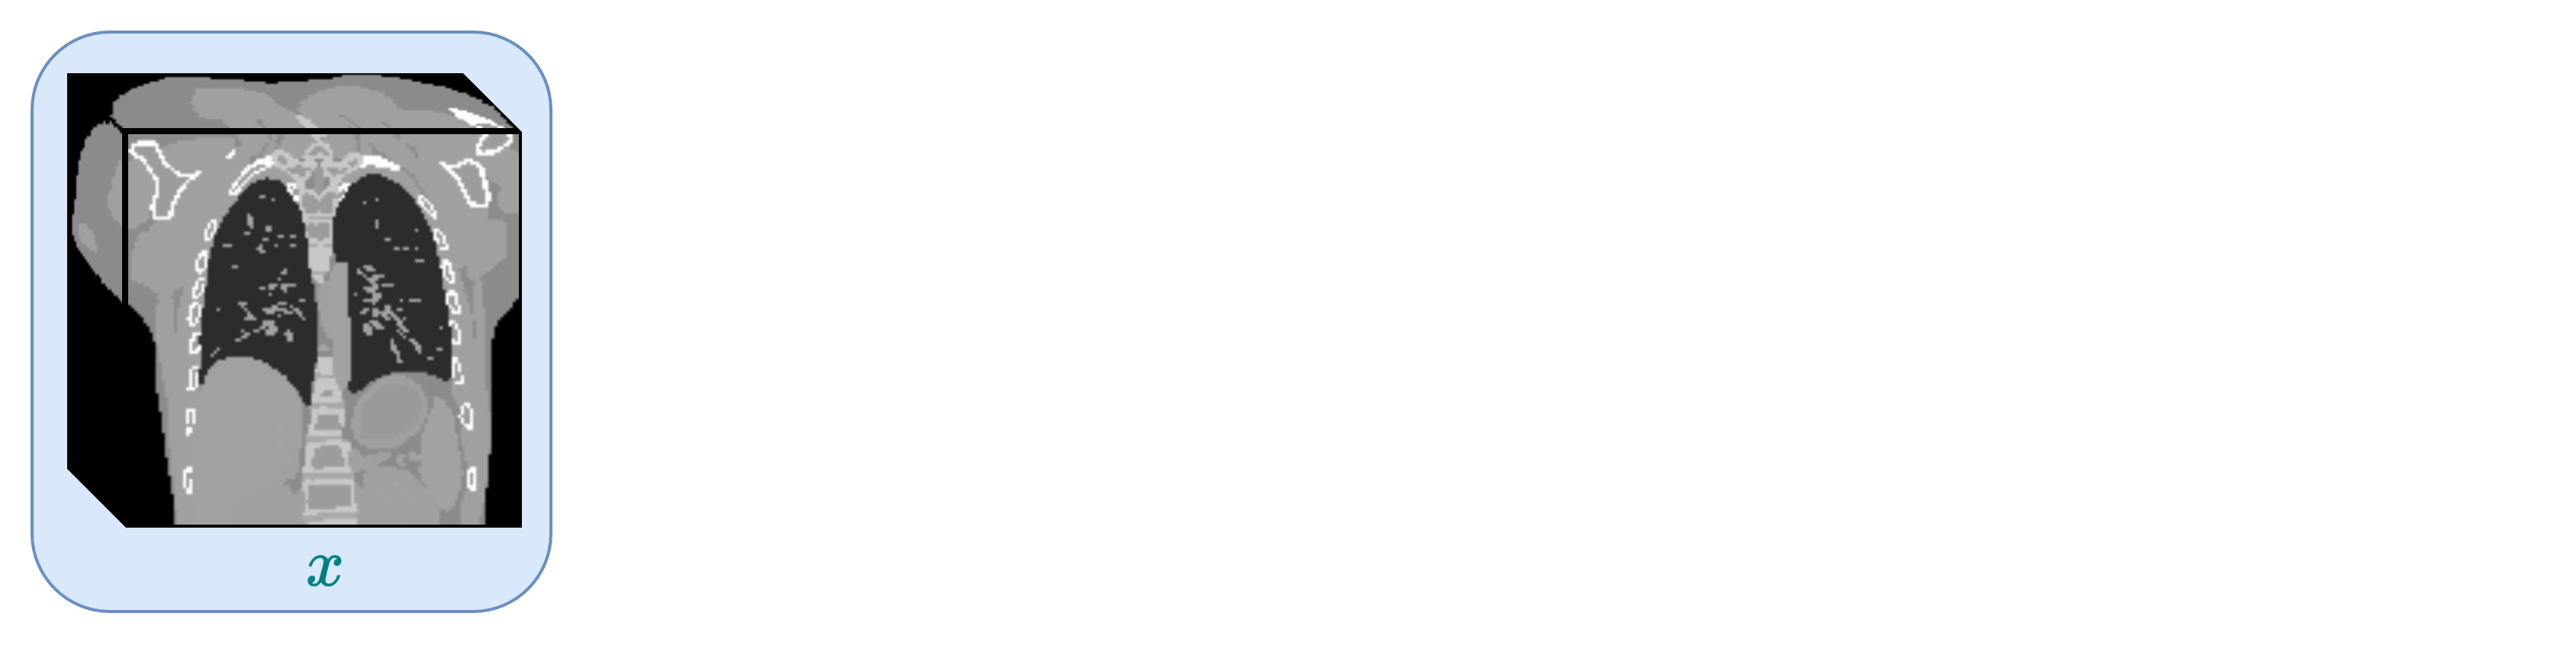
\includegraphics[width=1.0\linewidth]{figures/intro/blindforward/blindforward1.png}}
            \only<4>{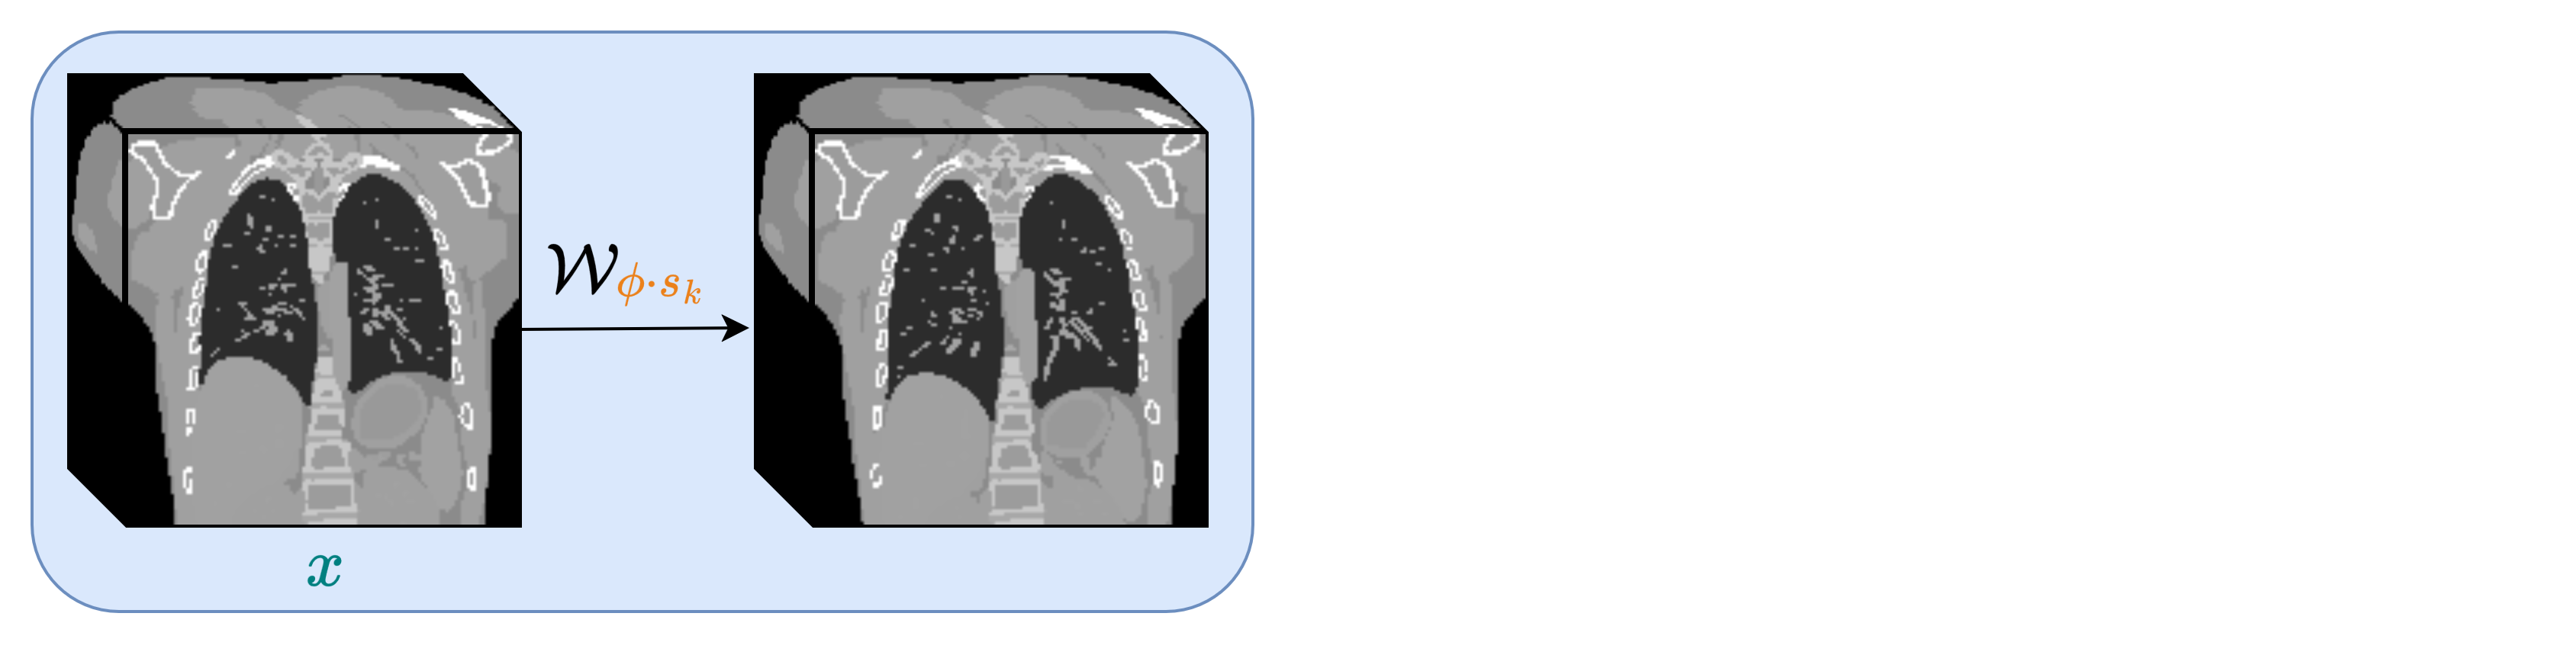
\includegraphics[width=1.0\linewidth]{figures/intro/blindforward/blindforward2.png}}
            \only<5>{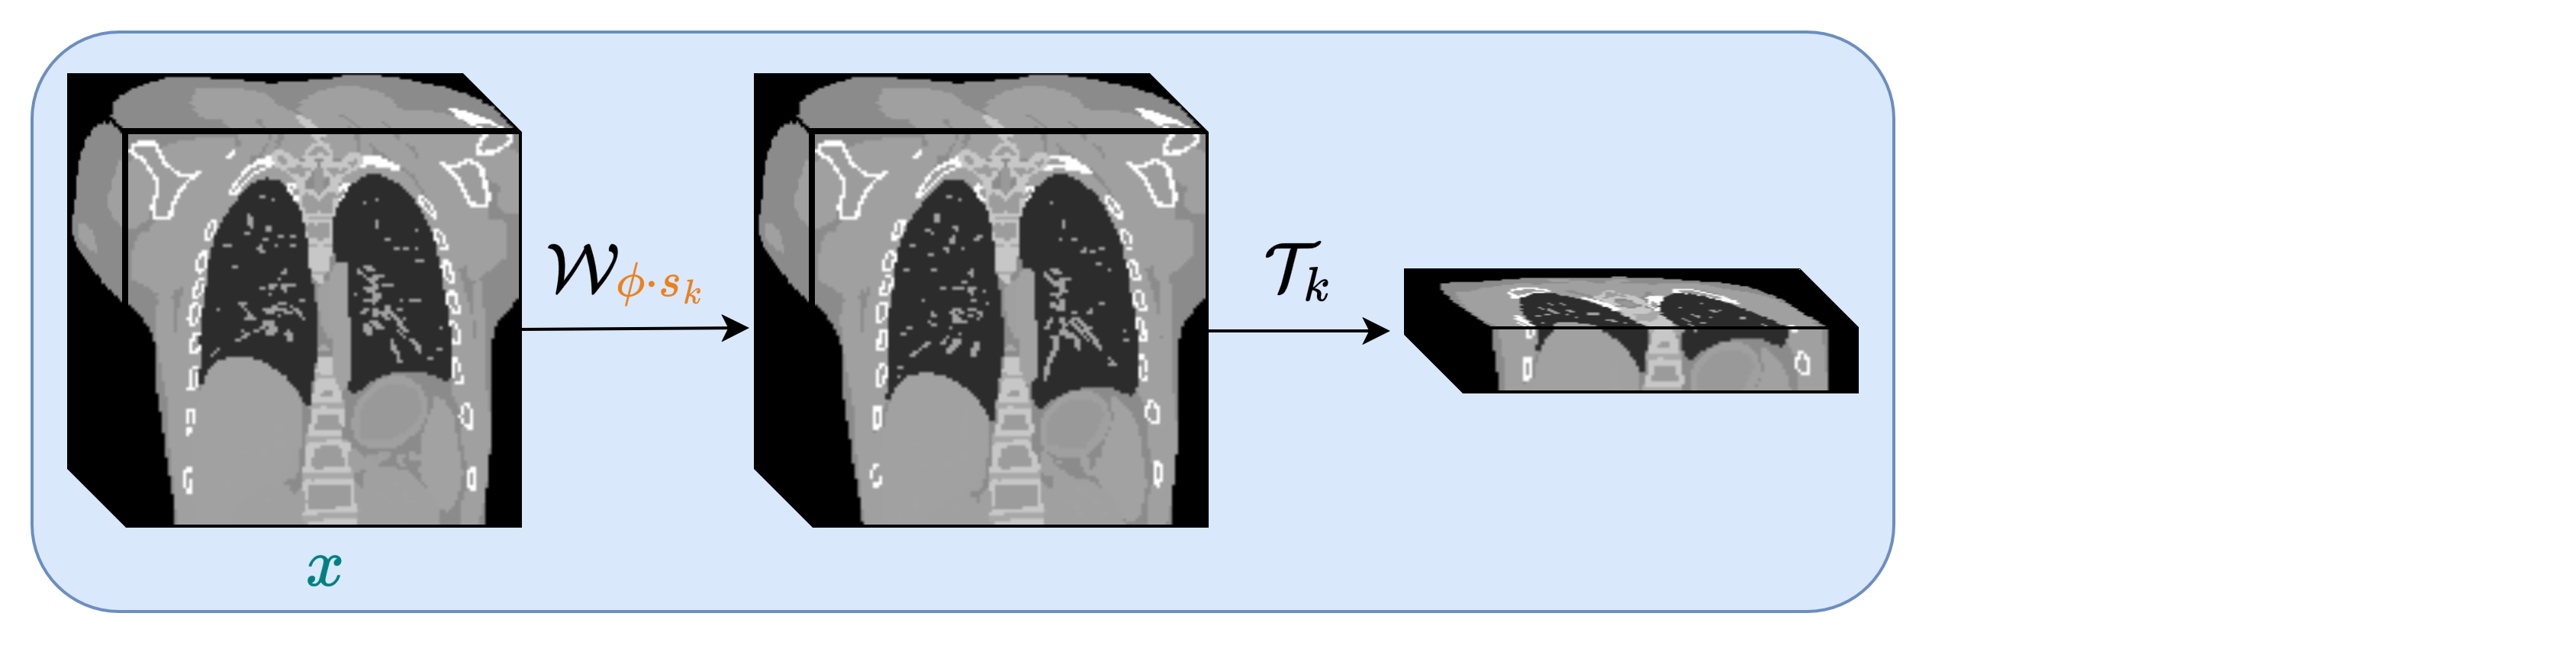
\includegraphics[width=1.0\linewidth]{figures/intro/blindforward/blindforward3.png}}
            \only<6>{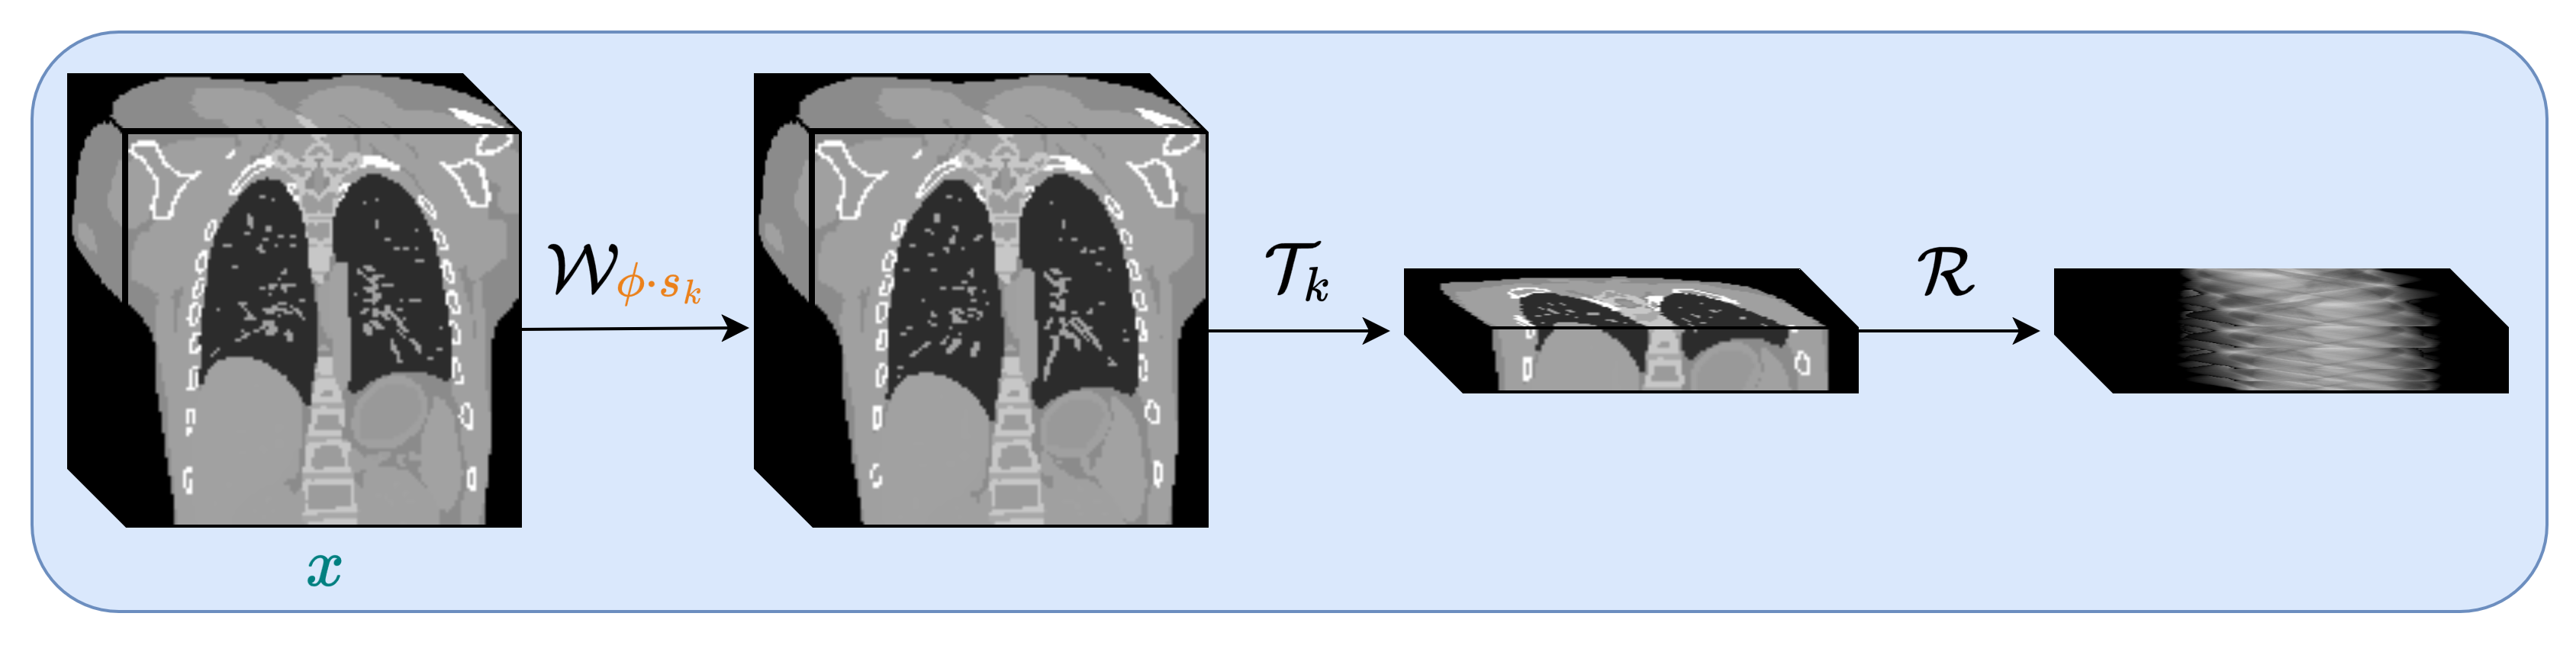
\includegraphics[width=1.0\linewidth]{figures/intro/blindforward/blindforward4.png}}
            where $\textcolor{orange}{\boldphi}, \textcolor{orange}{\bolds}$ are deformation vector fields parametrized by B-spline grid and surrogate signals.
            \vspace{0.5cm}
    \end{itemize}
\end{frame}

  \section{Methods}

\begin{frame}[t, fragile]
    \frametitle{Challenges and Proposed Solution}

    \begin{itemize}
        \item<1-> \textbf{Challenges:}
              \begin{itemize}
                  \item Sparse-view data increases the ill-posedness of the problem.
                  \item Hand-crafted regularizers (e.g., Total Variation) tend to oversmooth and erase subtle image features.
              \end{itemize}

        \item<2-> \textbf{Solution Overview:}
              \begin{itemize}
                  \item JRM via Adaptive Diffusion Models (ADMs).
                  \item Motion-free $\textcolor{green}{\boldx}$ is estimated via a Deep Posterior Sampling (DPS) approach \cite{zhu2023denoising}.
                  \item Motion parameters $\textcolor{orange}{\boldphi}, \textcolor{orange}{\bolds}$ are estimated through a classical optimization pipeline.
                  \item Wavelet Diffusion Models (WDMs) \cite{friedrich2024wdm} are used to enhance computational efficiency.
              \end{itemize}
    \end{itemize}
\end{frame}



\begin{frame}[fragile]
	\frametitle{Overview of JRM-ADM}
	
        \only<1>{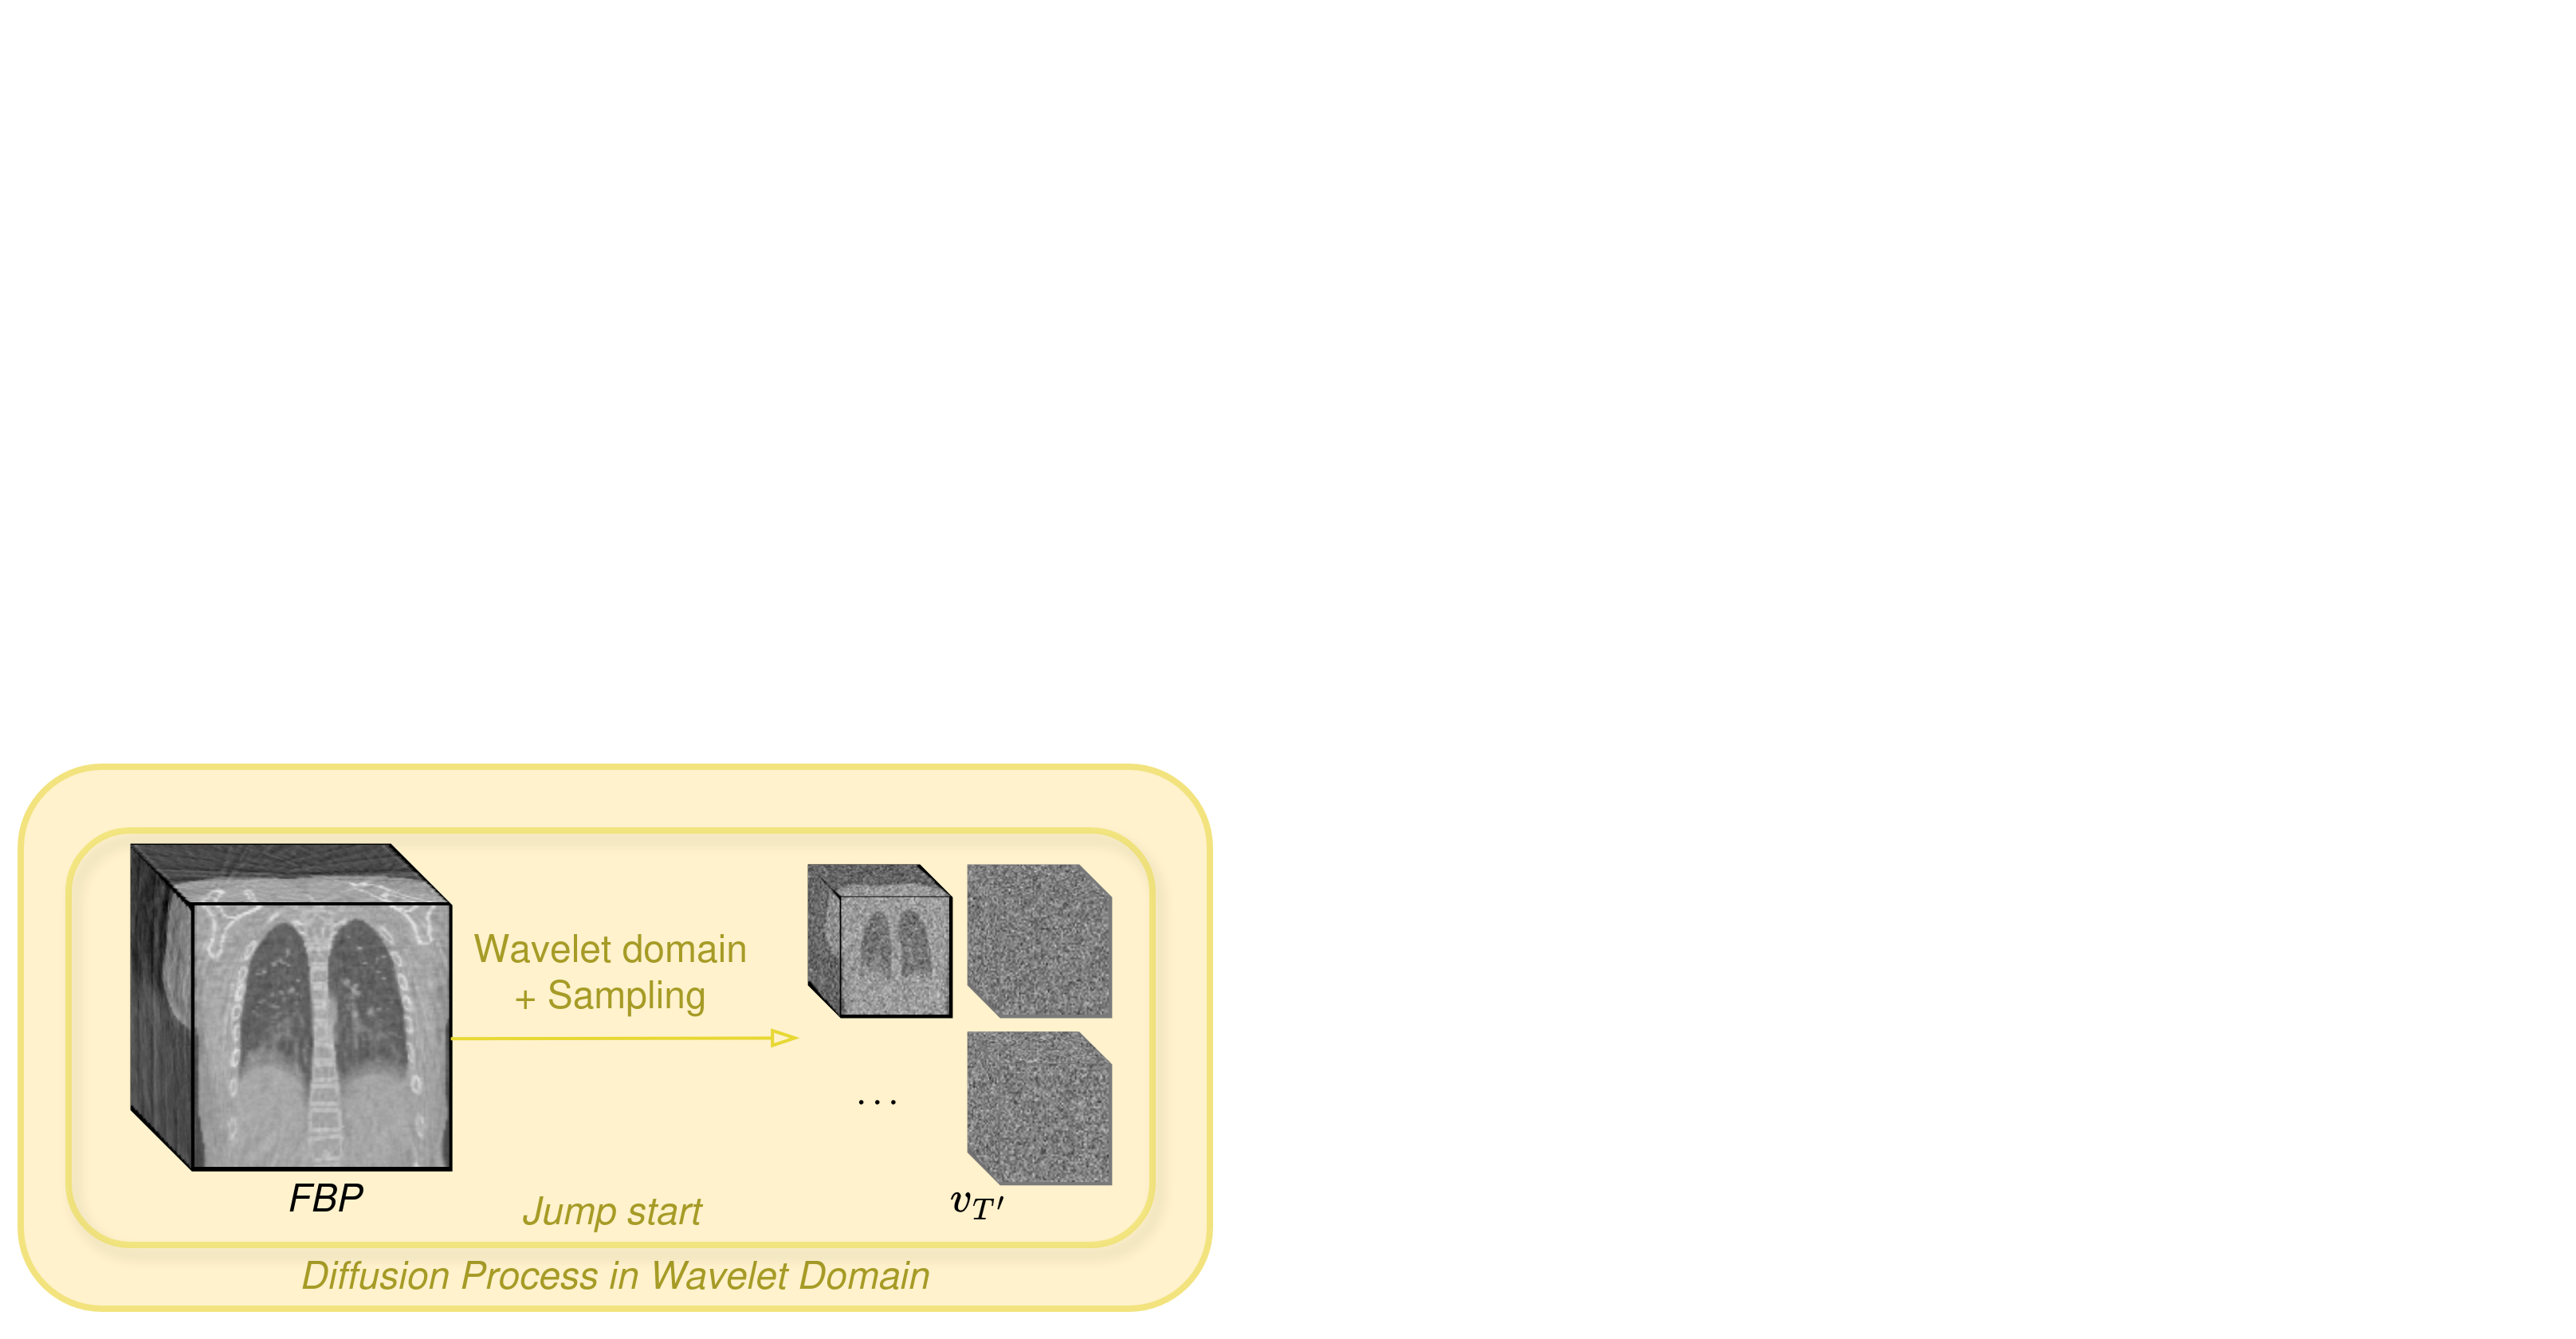
\includegraphics[width=1.0\linewidth]{figures/methods/overview/overview_1.png}}
        \only<2>{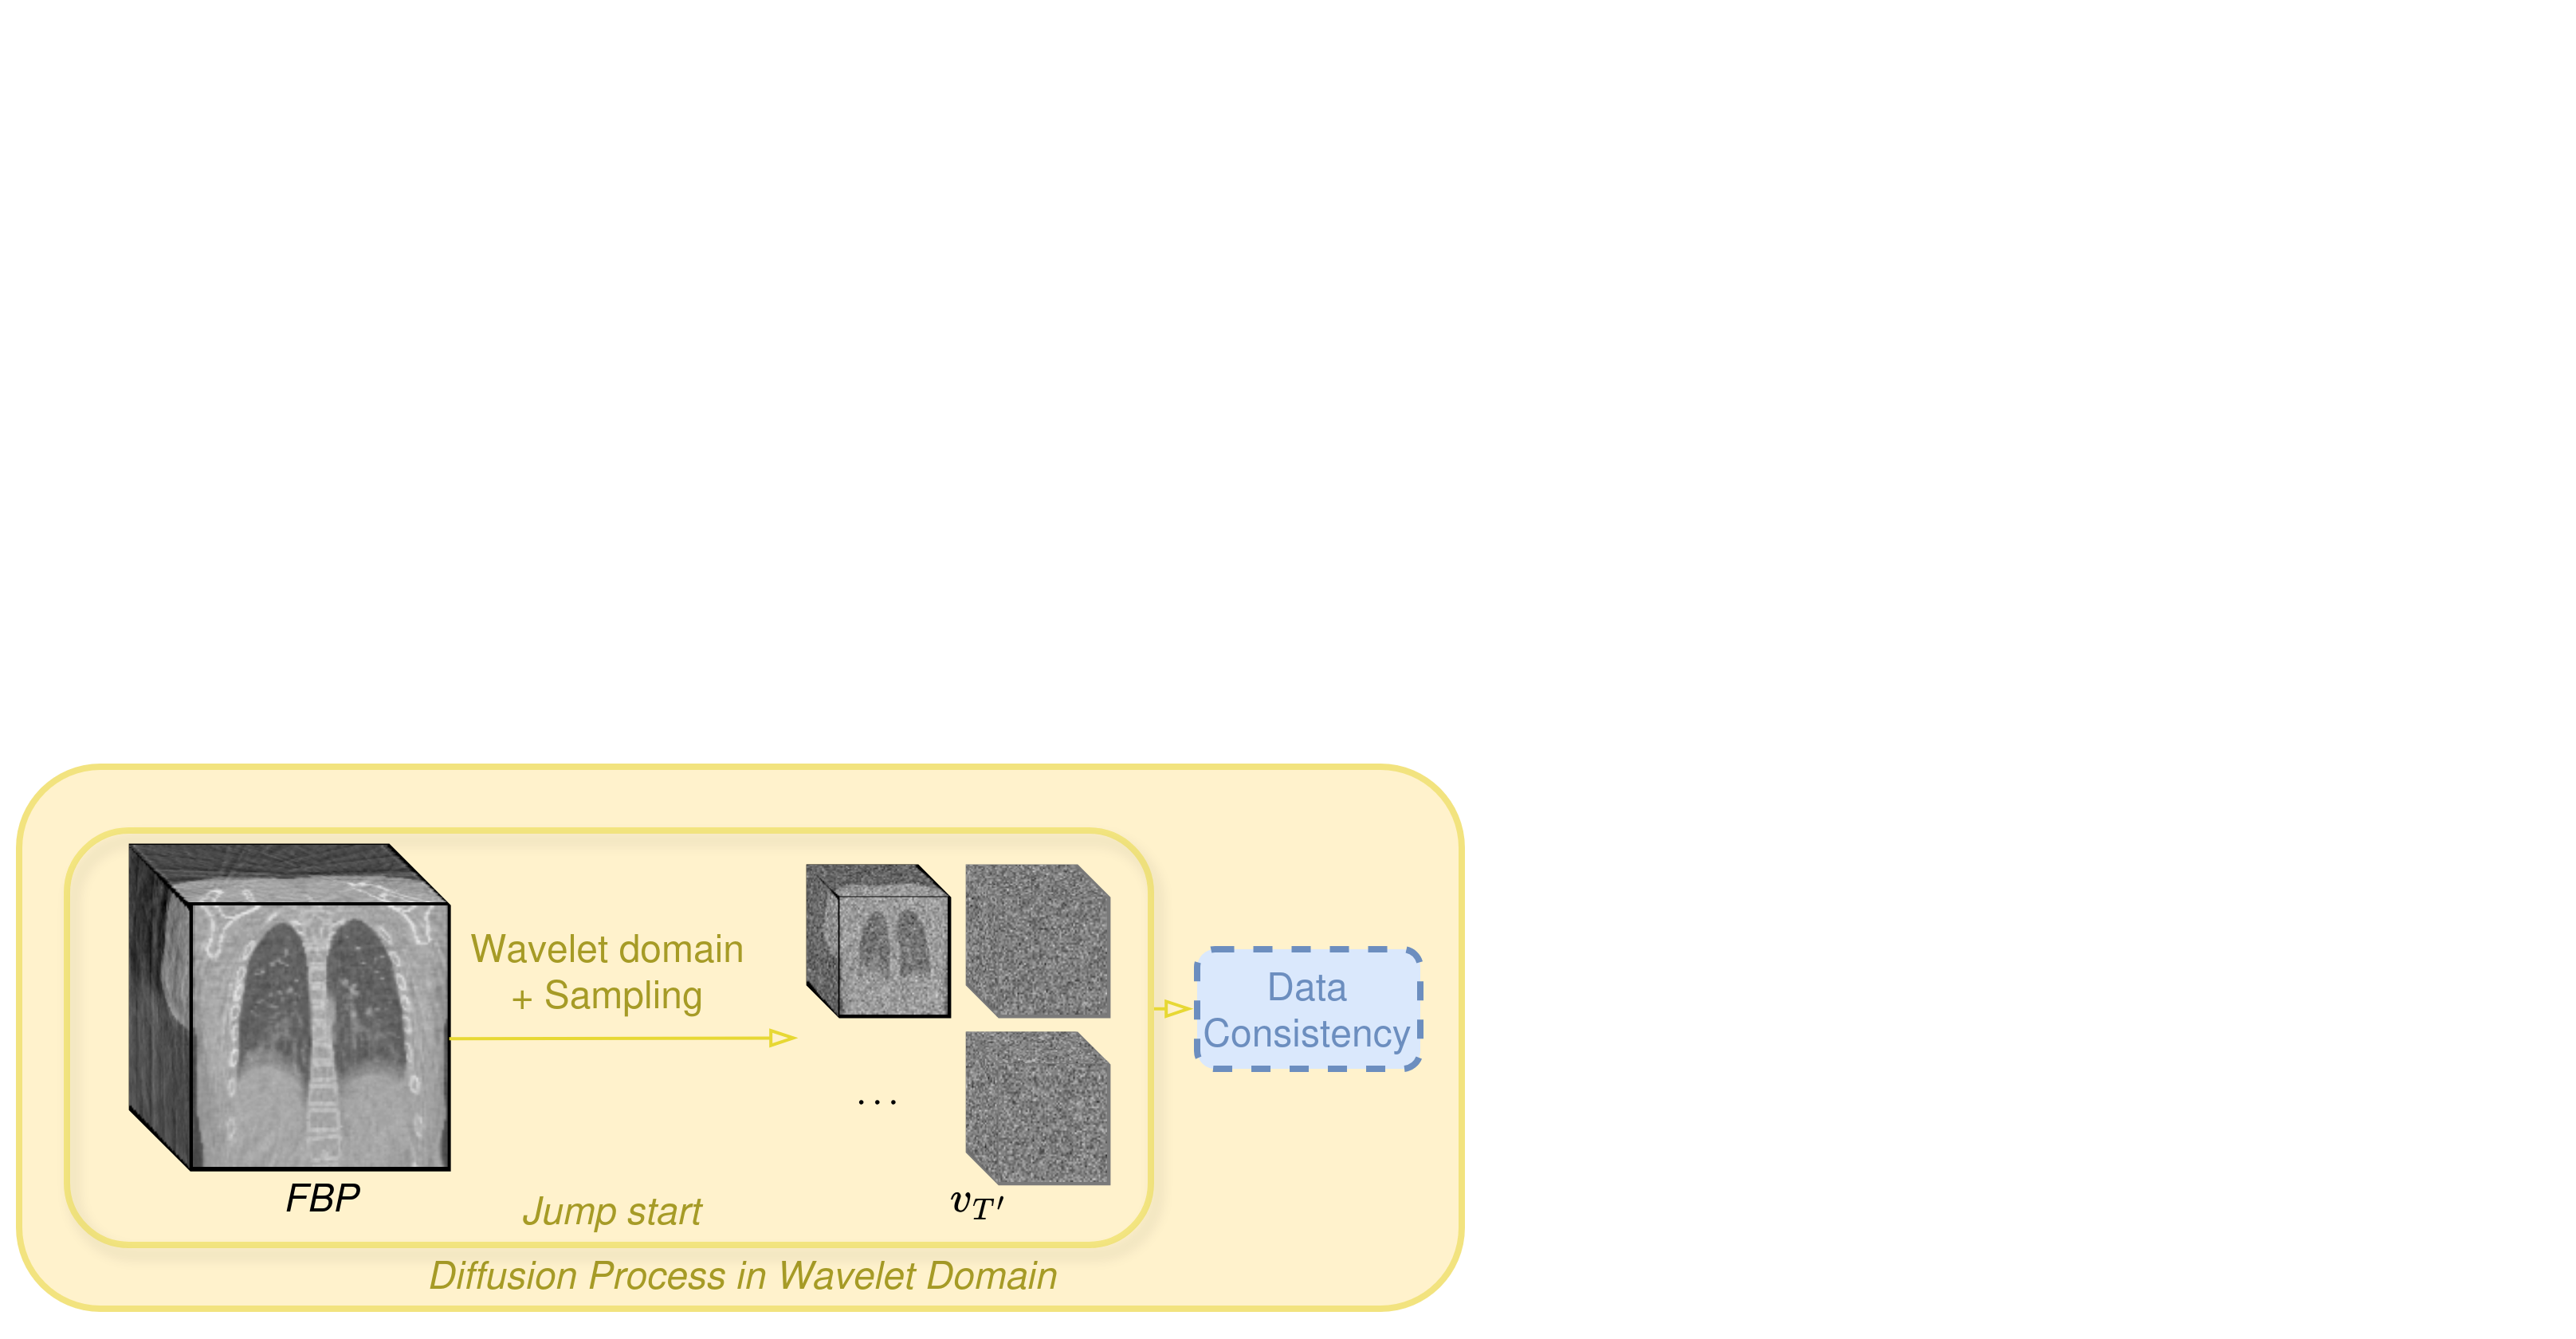
\includegraphics[width=1.0\linewidth]{figures/methods/overview/overview_2.png}}
        \only<3>{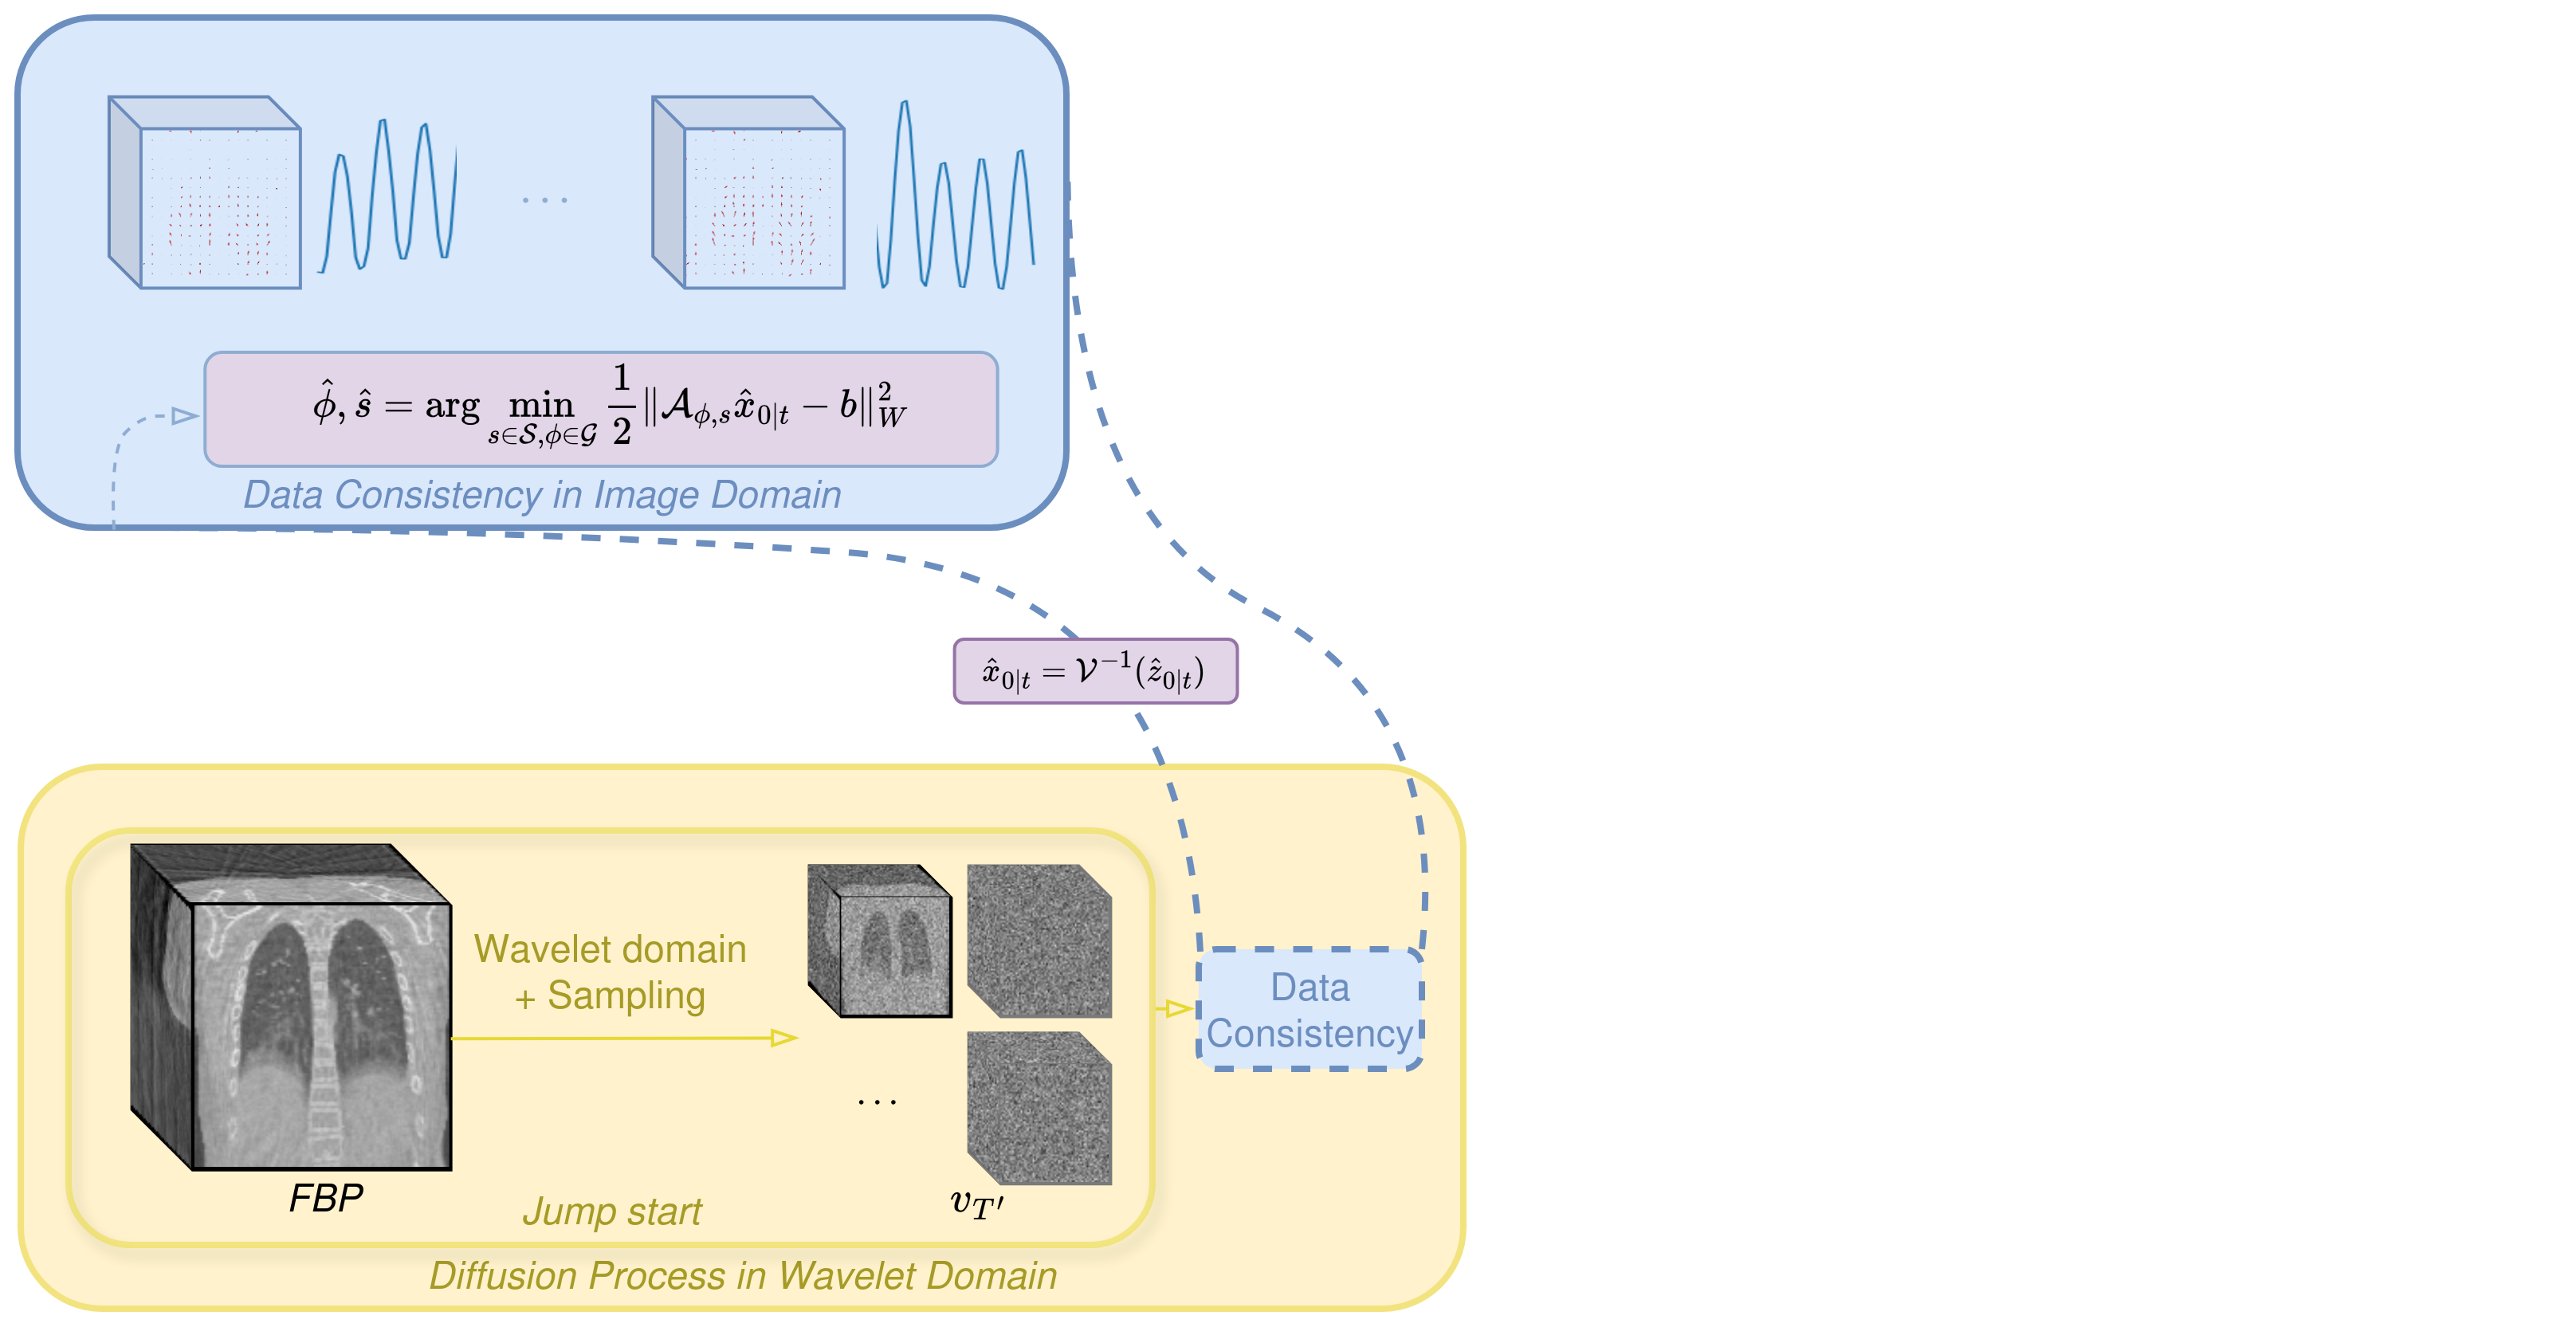
\includegraphics[width=1.0\linewidth]{figures/methods/overview/overview_3.png}}
        \only<4>{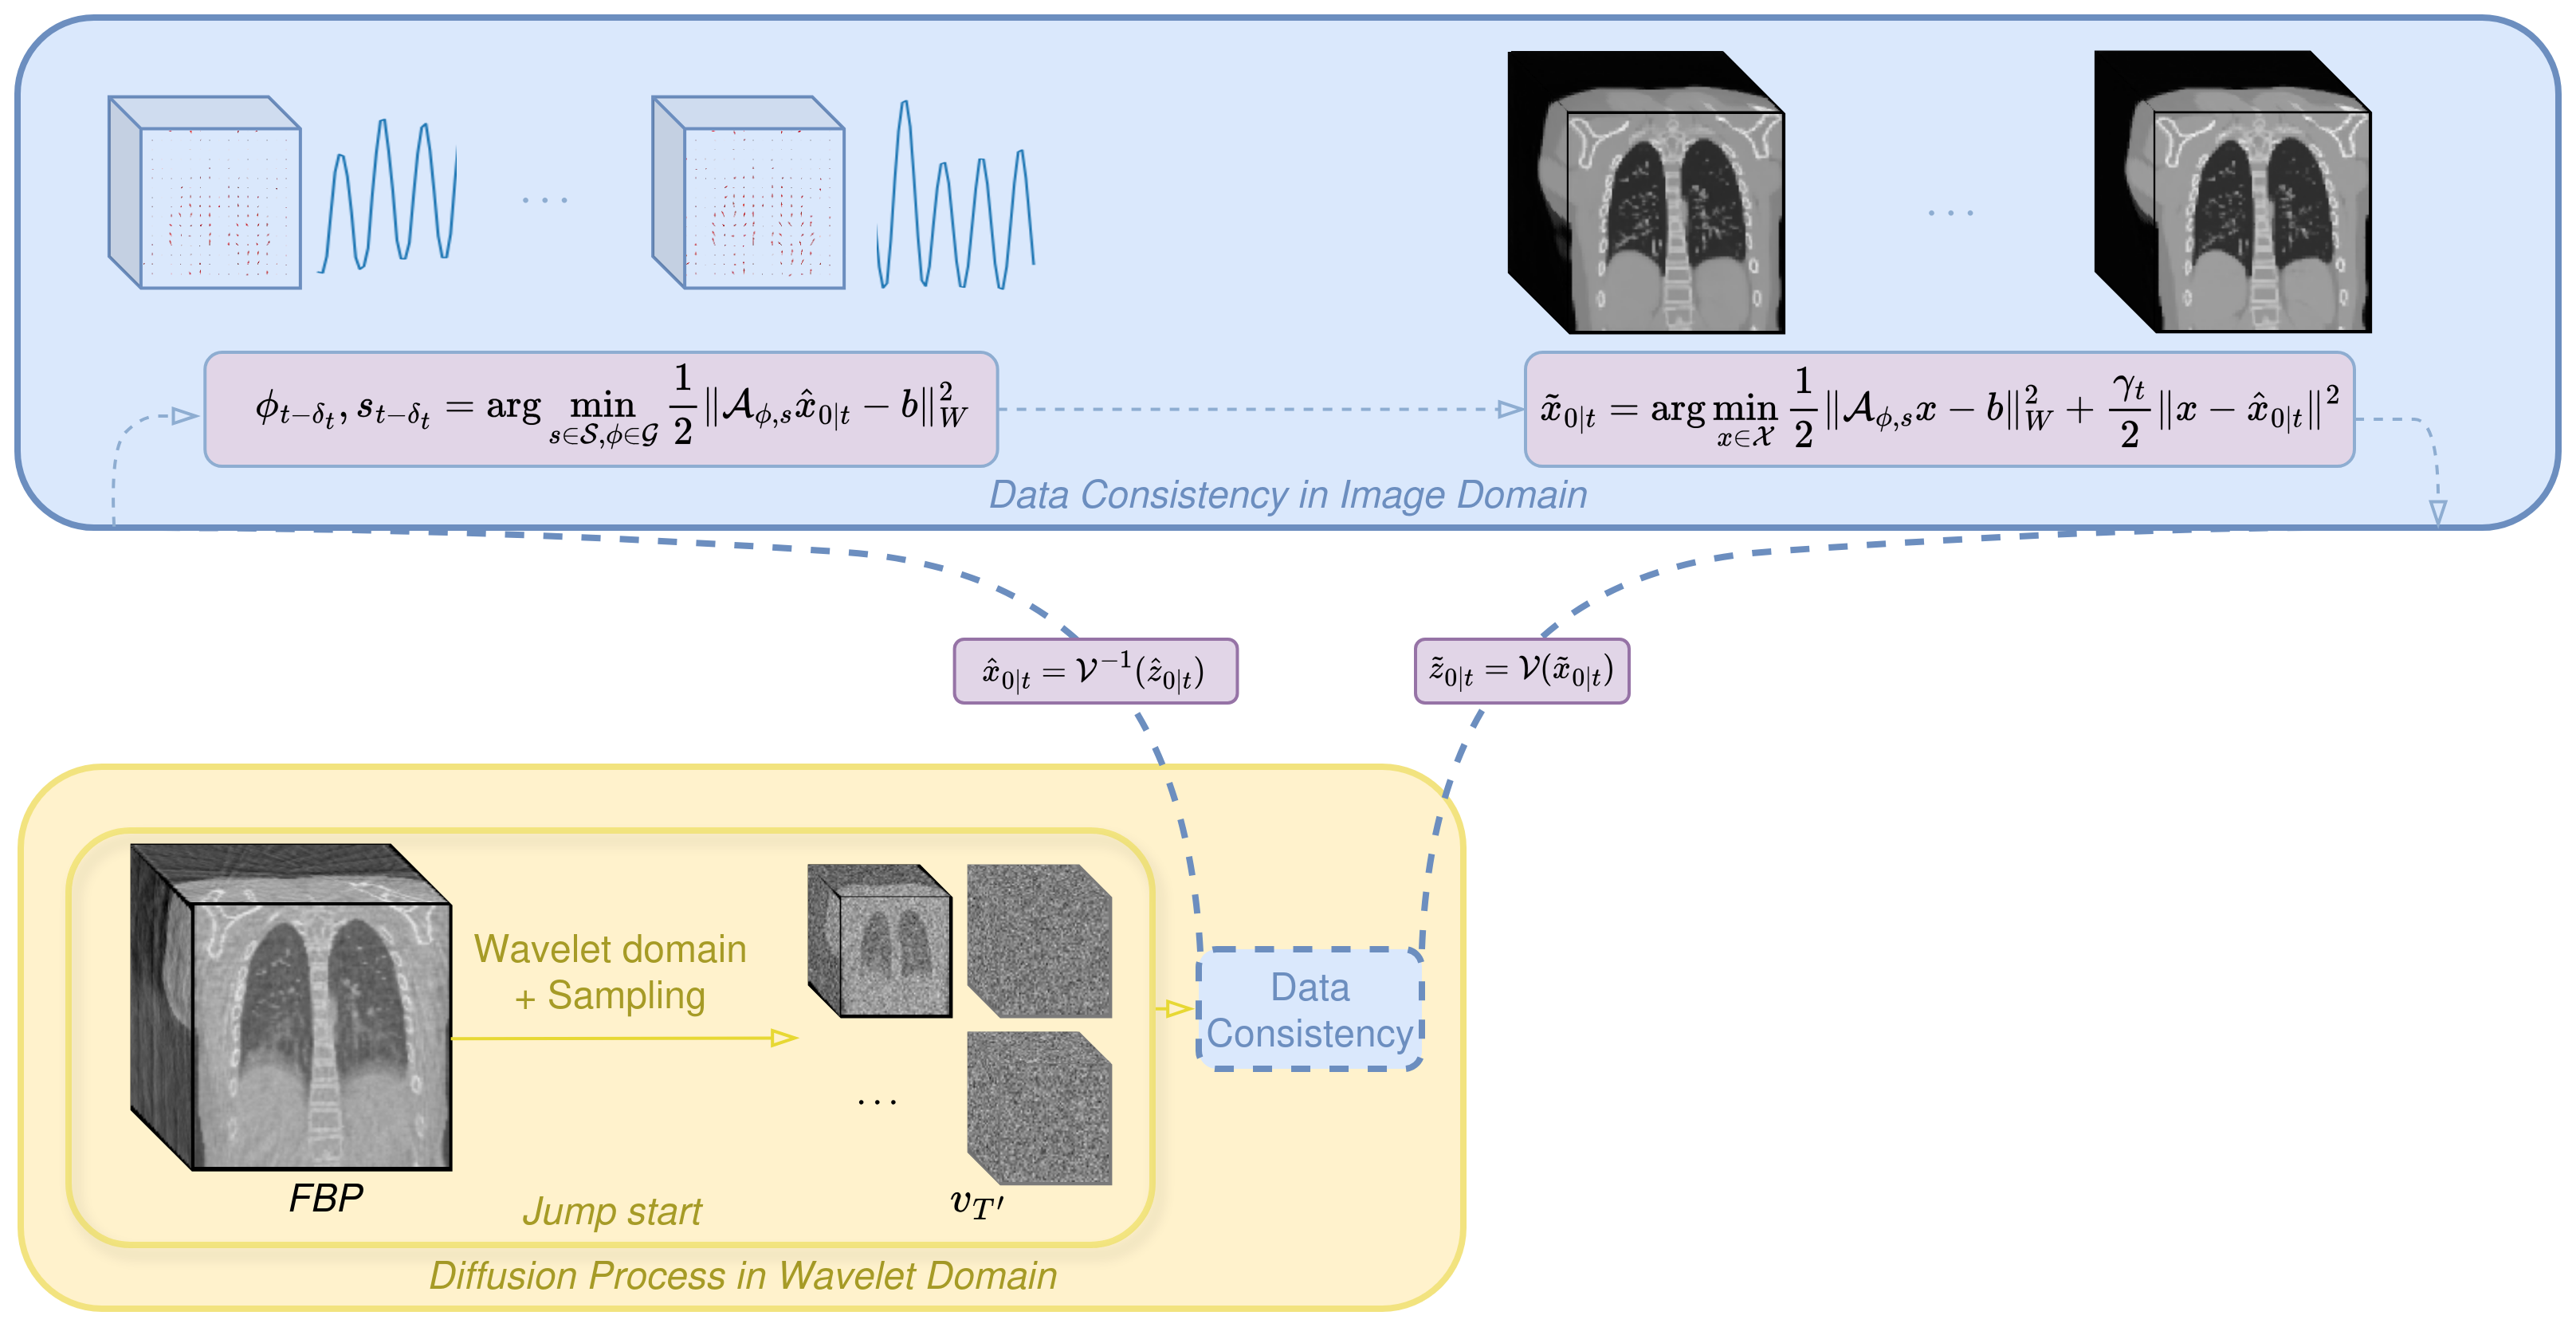
\includegraphics[width=1.0\linewidth]{figures/methods/overview/overview_4.png}}
        \only<5>{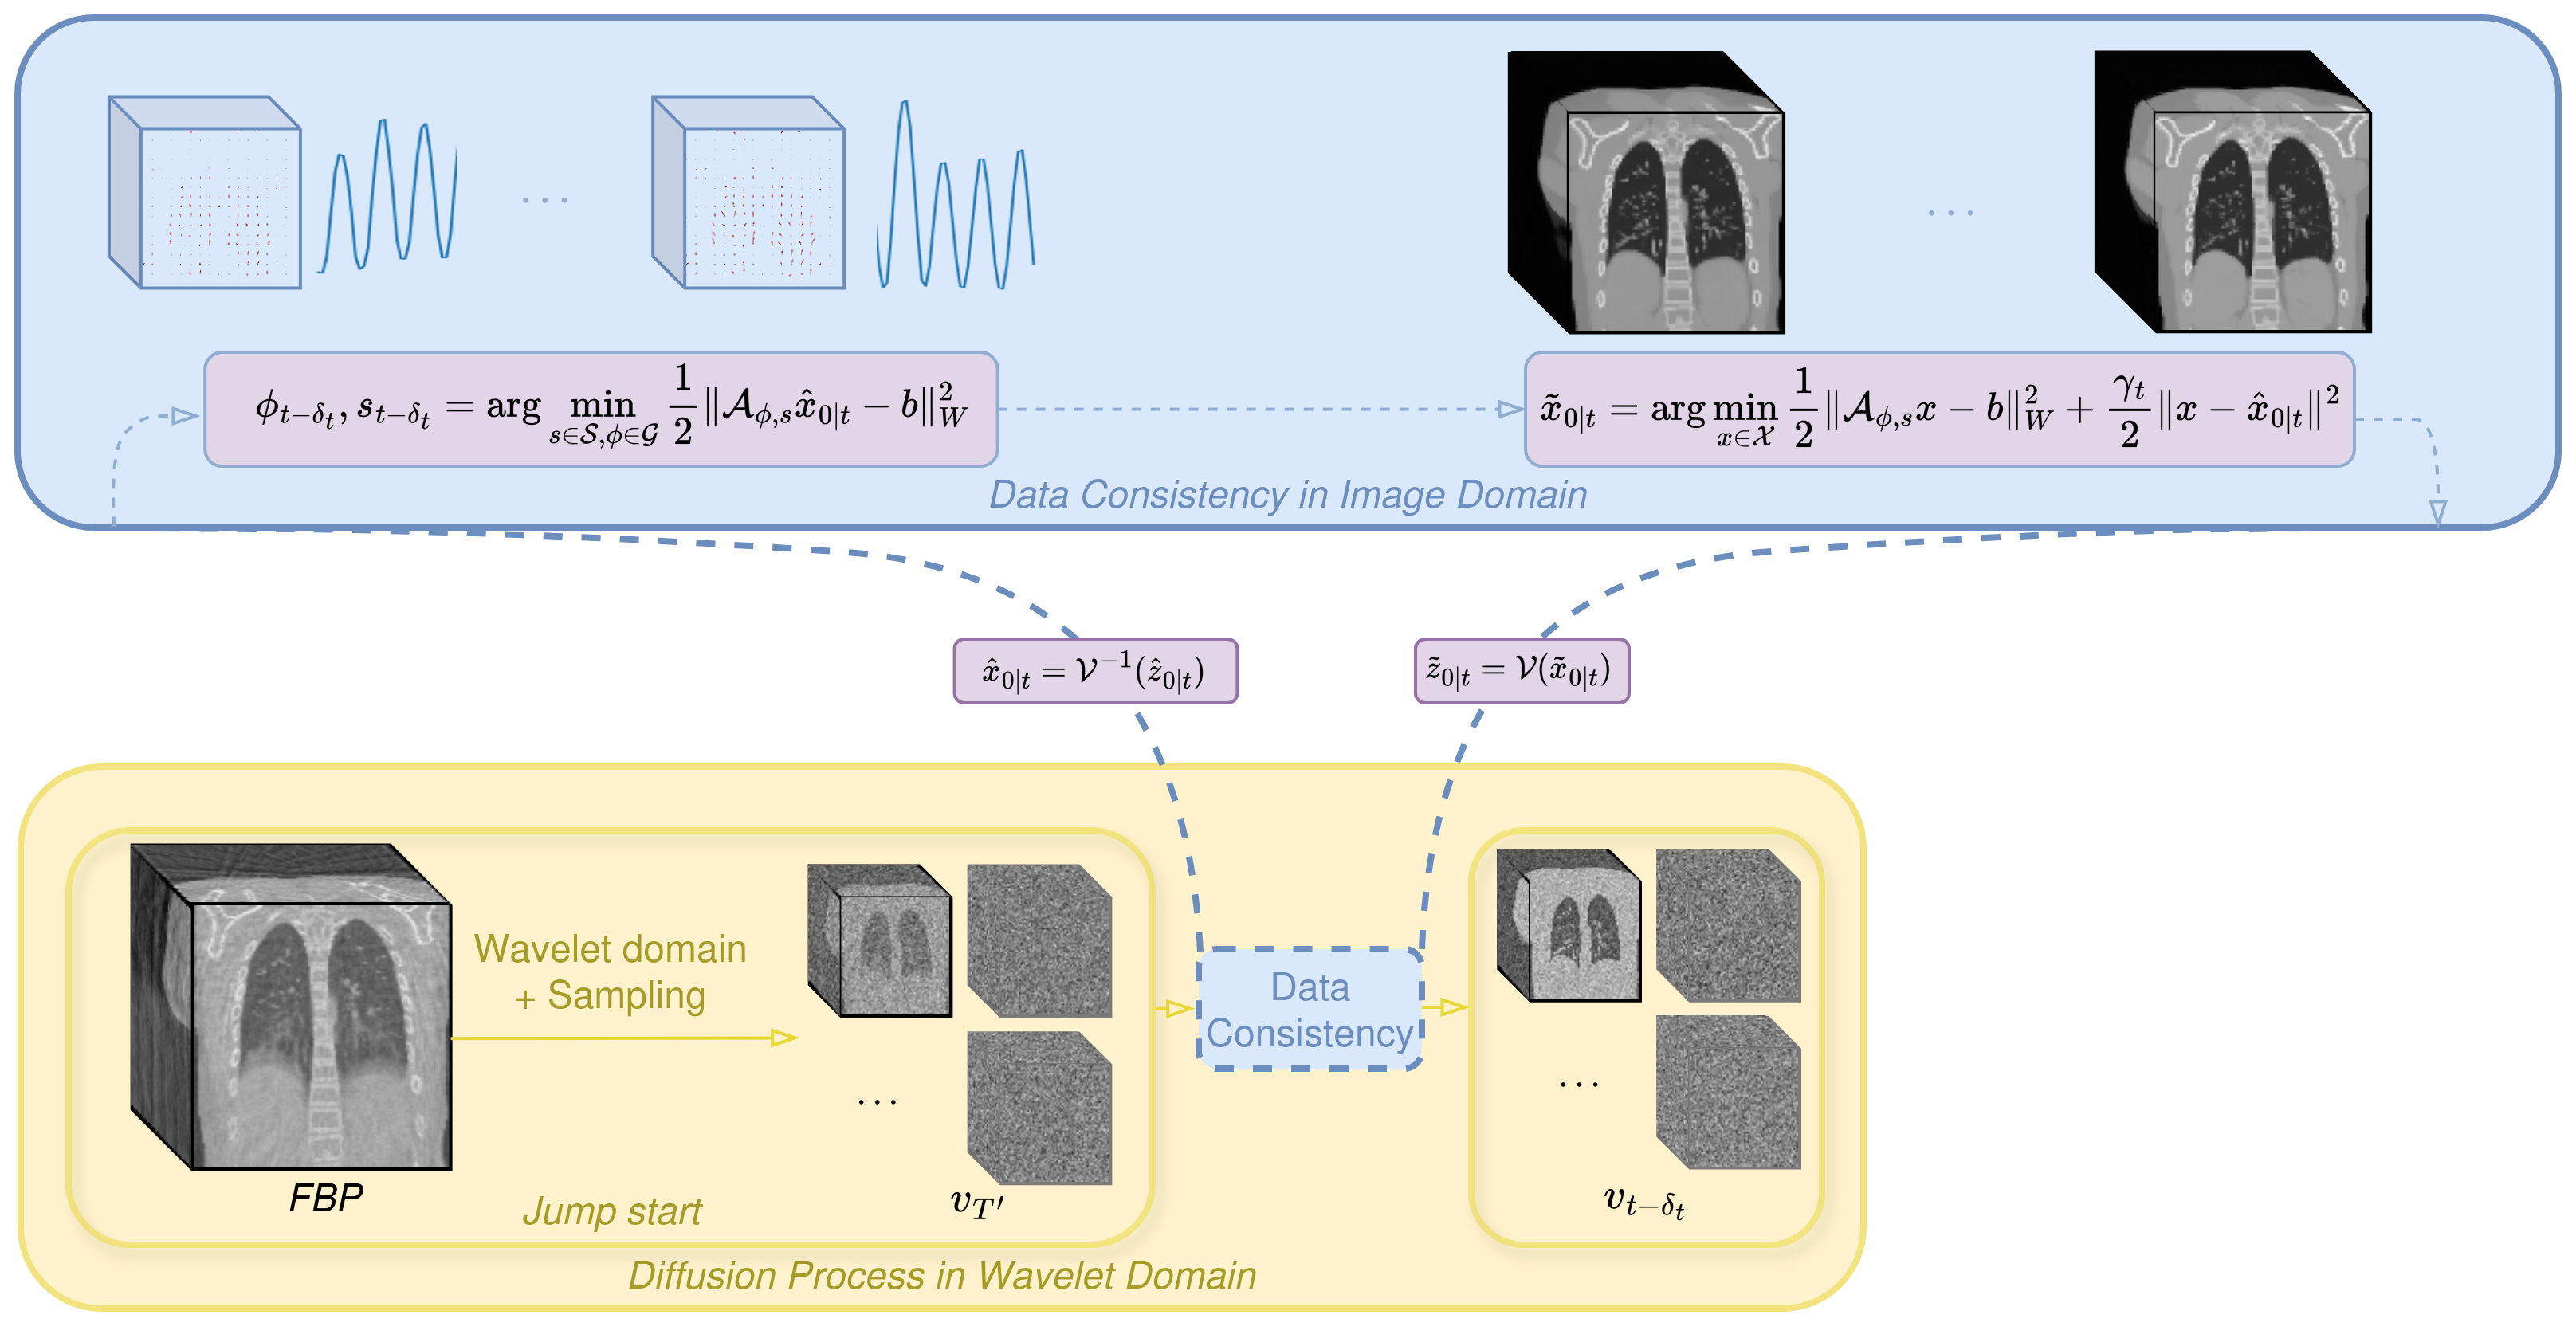
\includegraphics[width=1.0\linewidth]{figures/methods/overview/overview_5.png}}
        \only<6>{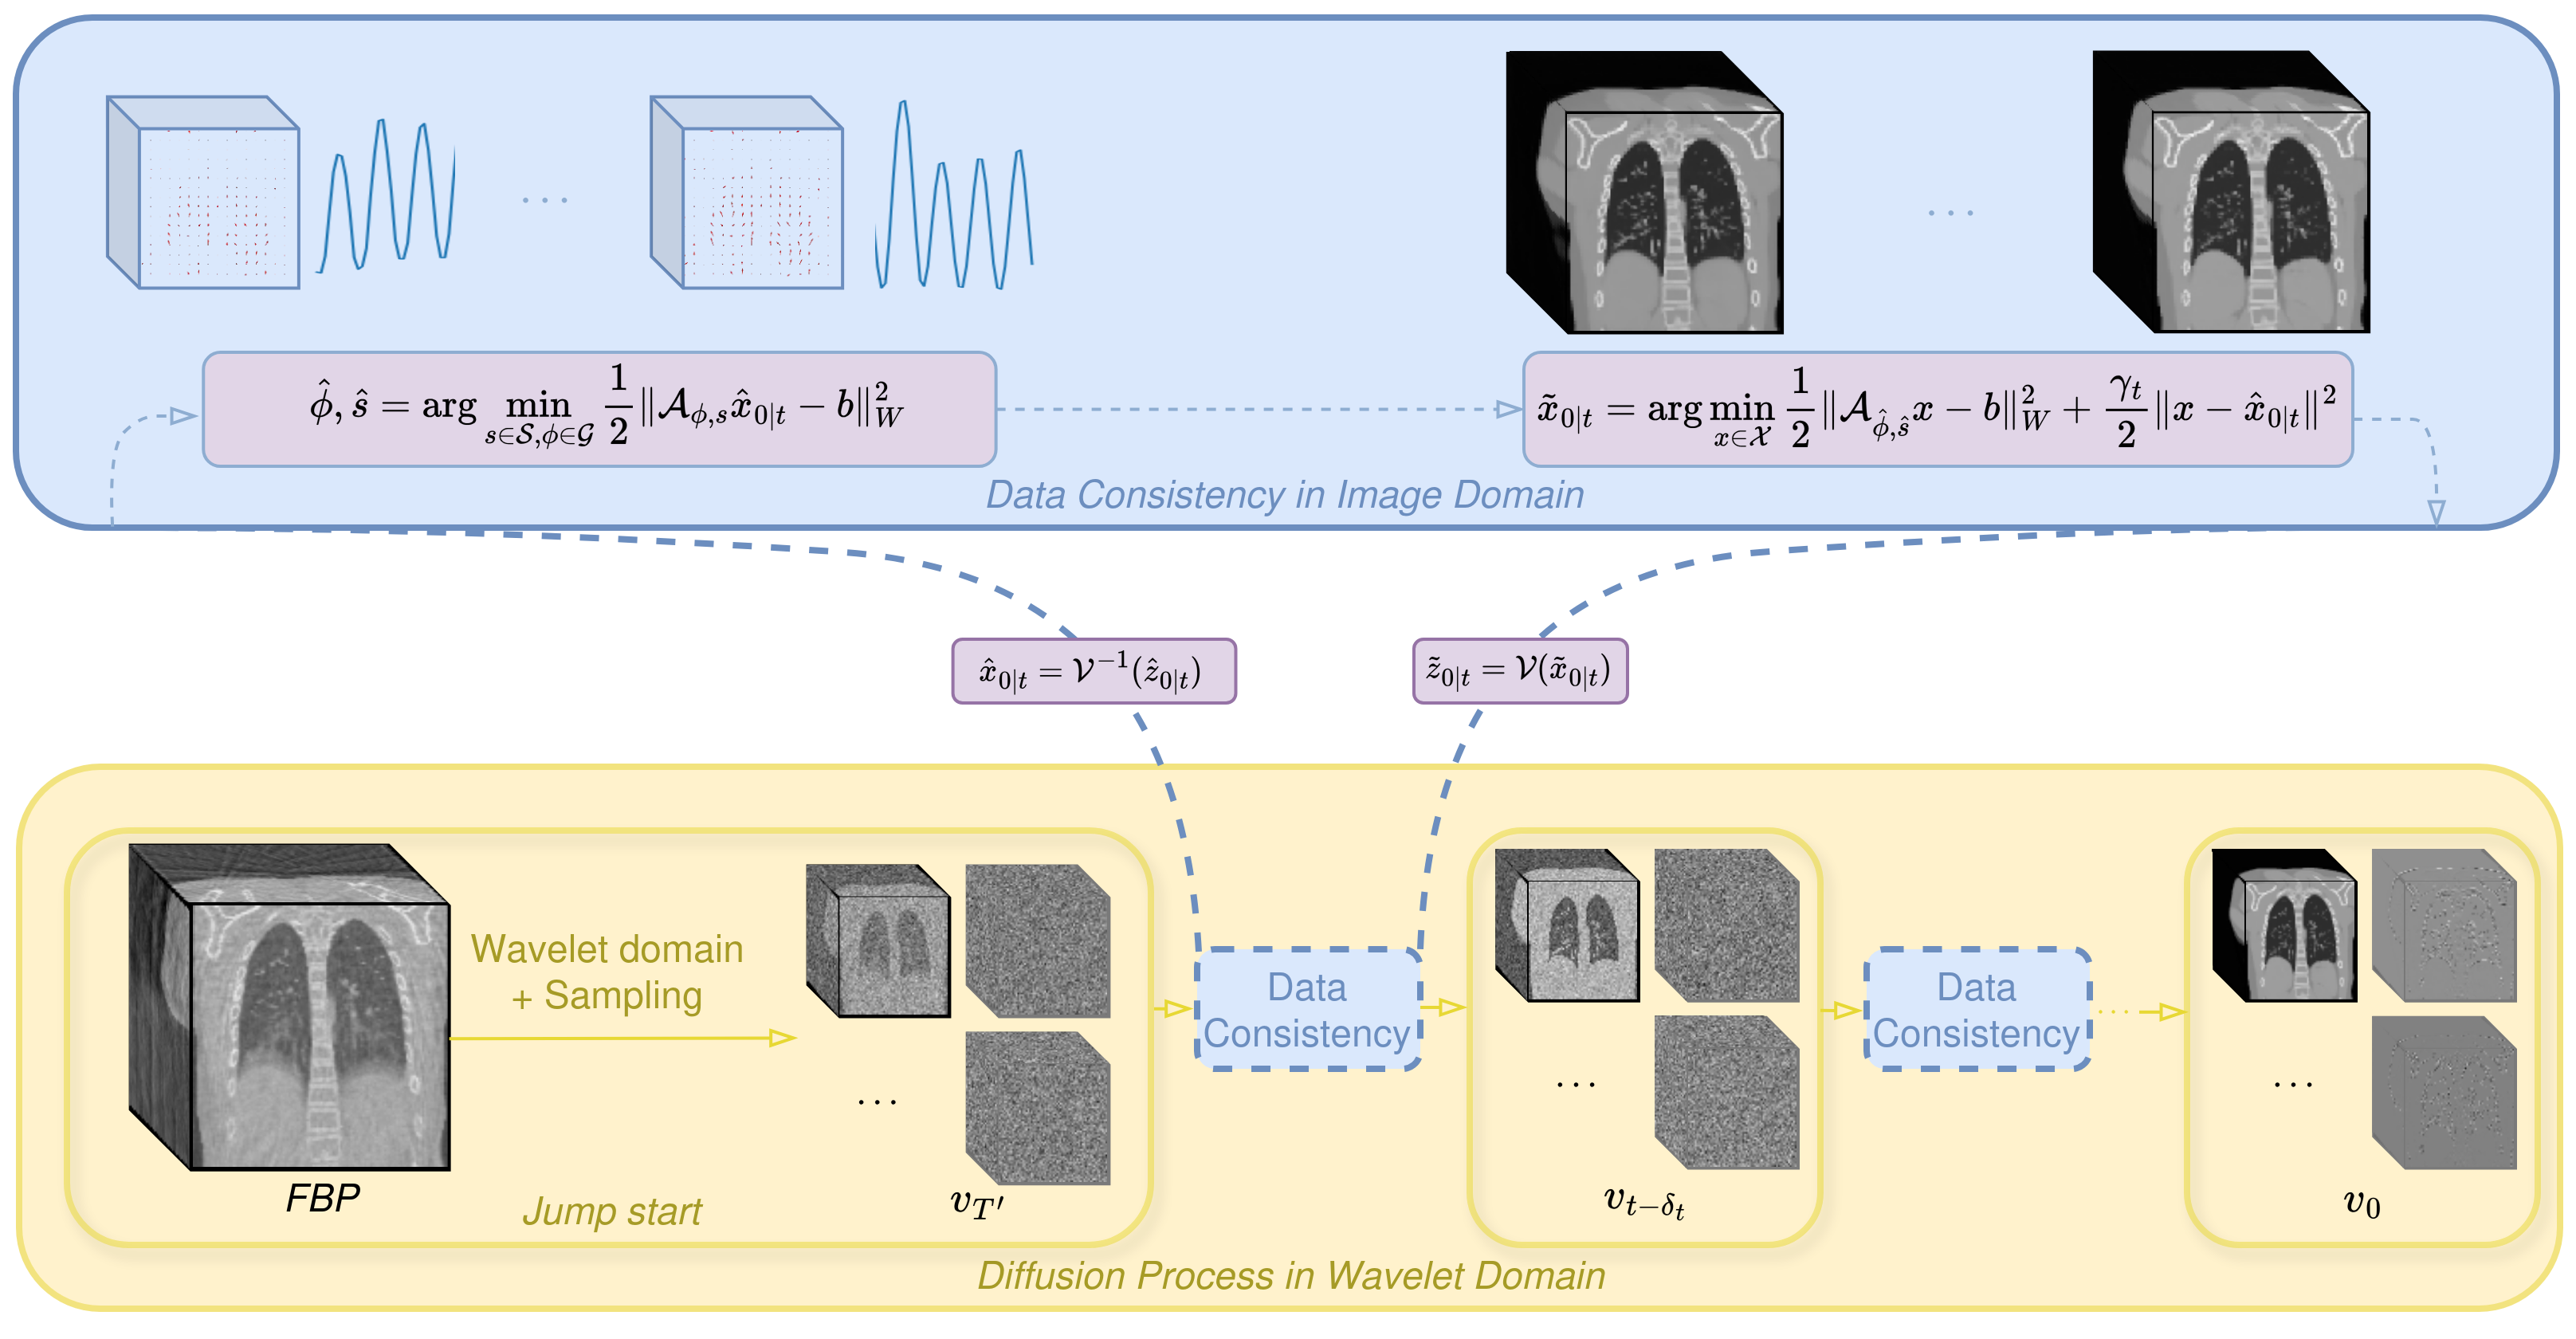
\includegraphics[width=1.0\linewidth]{figures/methods/overview/overview_6.png}}

\end{frame}
  % \begin{frame}[t, fragile]
%         \frametitle{Quantitative results}

%         \begin{columns}[T] % align columns at top
%                 \column{0.48\textwidth}
%                 \textbf{Experiments on XCAT Phantom:}
%                 \begin{itemize}
%                         \item<1-> Generated 3D thorax CT volumes (128$^3$ voxels, 2.6\,mm$^3$ voxel size) using the XCAT phantoms \cite{segars20104d}.
%                         \item<2-> Trained WDMs on these volumes to learn anatomical priors.
%                         \item<3-> Simulated sparse-view 4DCT acquisitions with 52 projection angles.
%                 \end{itemize}

%                 \column{0.48\textwidth}
%                 \textbf{Experiments on Pseudo-Real Data:}
%                 \begin{itemize}
%                         \item<4-> Using LIDC-IDRI \cite{armato2011lung} 3D thorax CT volumes (256$^3$ voxels, 1.25\,mm$^3$ voxel size)
%                         \item<5-> Trained WDMs on these volumes to learn anatomical priors.
%                         \item<6-> Simulated sparse-view 4DCT acquisitions on CHRU with 52 projection angles using a CT respiratory motion synthesis framework \cite{cao2024ct}.
%                 \end{itemize}
%         \end{columns}

%         \begin{itemize}
%                 \item<7-> \textbf{Evaluation:} Assessed reconstruction quality using metrics such as Structural Similarity Index (SSIM) and Peak Signal-to-Noise Ratio (PSNR).
%         \end{itemize}
% \end{frame}

\section{Experiments}




\begin{frame}[t,fragile]
  \frametitle{Quantitative Results}

  \begin{columns}[T]
    %─── Left column (shown on 1st overlay) ───
    \column{0.48\textwidth}
    \textbf{Experiments on XCAT Phantoms:}
    \begin{itemize}
      \item Generated 3D thorax CT volumes (128$^3$ voxels, 2.6\,mm$^3$ voxel size) using the XCAT phantoms \cite{segars20104d}.
      \item Trained WDMs on these volumes to learn anatomical priors.
      \item Simulated sparse-view 4DCT acquisitions with 52 projection angles.
    \end{itemize}

    \pause  % ← everything after this is hidden until the next click

    %─── Right column (shown on 2nd overlay) ───
    \column{0.48\textwidth}
    \textbf{Experiments on Pseudo-Real Data:}
    \begin{itemize}
      \item Using LIDC-IDRI \cite{armato2011lung} 3D thorax CT volumes (256$^3$ voxels, 1.25\,mm$^3$ voxel size)
      \item Trained WDMs on these volumes to learn anatomical priors.
      \item Simulated sparse-view 4DCT acquisitions on CHRU CT volumes with 52 projection angles using a CT respiratory motion synthesis framework \cite{cao2024ct}.
    \end{itemize}
  \end{columns}

  % you can still use \pause (or overlay specs) for the evaluation bullet
  \pause
  \begin{itemize}
    \item \textbf{Evaluation:} Assessed reconstruction quality using metrics such as SSIM and PSNR.
  \end{itemize}
\end{frame}


\begin{frame}[fragile]
        \frametitle{Quantitative Evaluation of Reconstruction Methods}

        \begin{table}[ht]
                \centering
                \renewcommand{\arraystretch}{1.2} % Adjust row height
                \setlength{\tabcolsep}{6pt}       % Adjust column spacing
                \footnotesize                     % Set font size for the table
                \begin{tabular}{lcccc}
                        \toprule
                        \textbf{Metric}          & \textbf{Gated FBP} & \textbf{Gated DPS} & \textbf{JRM-TV} & \textbf{JRM-ADM} \\
                        \midrule
                        \textbf{PSNR} $\uparrow$ & 20.59              & 24.09              & 25.04           & \textbf{27.05}   \\
                        \textbf{SSIM} $\uparrow$ & 0.37               & 0.90               & 0.89            & \textbf{0.94}    \\
                        \bottomrule
                \end{tabular}
                \caption{Quantitative evaluation (PSNR, SSIM) of four different reconstruction methods on the end-inhale phase for five XCAT phantoms.}
        \end{table}
\end{frame}



\begin{frame}[fragile]
        \frametitle{Qualitative Evaluation of Reconstruction Methods}

        \newlength{\tempdima}
        \setlength{\tempdima}{0.16\linewidth}



        \begin{figure}
                \centering

               
                \begin{subfigure}{0.19\linewidth}
                        \begin{tikzpicture}
                                \begin{scope}[spy using outlines={rounded rectangle, magnification=2, width=1.0cm, height=0.75cm, connect spies}]
                                        \node[inner sep=0pt] {
                                                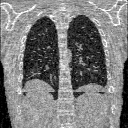
\includegraphics[width=\tempdima,height=\tempdima]{figures/experiments/xcat/fbp_coronal.png}
                                        };
                                        \spy [yellow] on (0.35,-0.3) in node [left,yellow] at (1.2, 1.0);
                                \end{scope}
                        \end{tikzpicture}
                \end{subfigure}
                \begin{subfigure}{0.19\linewidth}
                        \begin{tikzpicture}
                                \begin{scope}[spy using outlines={rounded rectangle, magnification=2, width=1.0cm, height=0.75cm, connect spies}]
                                        \node[inner sep=0pt] {
                                                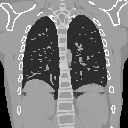
\includegraphics[width=\tempdima,height=\tempdima]{figures/experiments/xcat/gated_dps_coronal.png}
                                        };
                                        \spy [yellow] on (0.35,-0.3) in node [left,yellow] at (1.2, 1.0);
                                \end{scope}
                        \end{tikzpicture}
                \end{subfigure}
                \begin{subfigure}{0.19\linewidth}
                        \begin{tikzpicture}
                                \begin{scope}[spy using outlines={rounded rectangle, magnification=2, width=1.0cm, height=0.75cm, connect spies}]
                                        \node[inner sep=0pt] {
                                                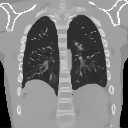
\includegraphics[width=\tempdima,height=\tempdima]{figures/experiments/xcat/blind_tv_coronal.png}
                                        };
                                        \spy [yellow] on (0.35,-0.3) in node [left,yellow] at (1.2, 1.0);
                                \end{scope}
                        \end{tikzpicture}
                \end{subfigure}
                \begin{subfigure}{0.19\linewidth}
                        \begin{tikzpicture}
                                \begin{scope}[spy using outlines={rounded rectangle, magnification=2, width=1.0cm, height=0.75cm, connect spies}]
                                        \node[inner sep=0pt] {
                                                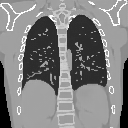
\includegraphics[width=\tempdima,height=\tempdima]{figures/experiments/xcat/blind_dps_coronal.png}
                                        };
                                        \spy [yellow] on (0.35,-0.3) in node [left,yellow] at (1.2, 1.0);
                                \end{scope}
                        \end{tikzpicture}
                \end{subfigure}
                \begin{subfigure}{0.19\linewidth}
                        \begin{tikzpicture}
                                \begin{scope}[spy using outlines={rounded rectangle, magnification=2, width=1.0cm, height=0.75cm, connect spies}]
                                        \node[inner sep=0pt] {
                                                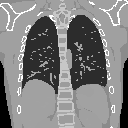
\includegraphics[width=\tempdima,height=\tempdima]{figures/experiments/xcat/gt_coronal.png}
                                        };
                                        \spy [yellow] on (0.35,-0.3) in node [left,yellow] at (1.2, 1.0);
                                \end{scope}
                        \end{tikzpicture}
                \end{subfigure}


                \begin{subfigure}{0.19\linewidth}
                        \begin{tikzpicture}
                                \begin{scope}[spy using outlines={rounded rectangle, magnification=2, width=1.0cm, height=0.75cm, connect spies}]
                                        \node[inner sep=0pt] {
                                                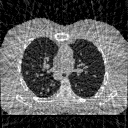
\includegraphics[width=\tempdima,height=\tempdima]{figures/experiments/xcat/fbp_axial.png}
                                        };
                                        \spy [yellow] on (0.05,-0.4) in node [left,yellow] at (1.2, 1.0);
                                \end{scope}
                        \end{tikzpicture}
                        \caption{\scriptsize Gated FBP}
                \end{subfigure}
                \begin{subfigure}{0.19\linewidth}
                        \begin{tikzpicture}
                                \begin{scope}[spy using outlines={rounded rectangle, magnification=2, width=1.0cm, height=0.75cm, connect spies}]
                                        \node[inner sep=0pt] {
                                                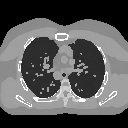
\includegraphics[width=\tempdima,height=\tempdima]{figures/experiments/xcat/gated_dps_axial.png}
                                        };
                                        \spy [yellow] on (0.05,-0.4) in node [left,yellow] at (1.2, 1.0);
                                \end{scope}
                        \end{tikzpicture}
                        \caption{\scriptsize Gated DPS}
                \end{subfigure}
                \begin{subfigure}{0.19\linewidth}
                        \begin{tikzpicture}
                                \begin{scope}[spy using outlines={rounded rectangle, magnification=2, width=1.0cm, height=0.75cm, connect spies}]
                                        \node[inner sep=0pt] {
                                                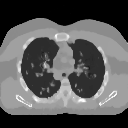
\includegraphics[width=\tempdima,height=\tempdima]{figures/experiments/xcat/blind_tv_axial.png}
                                        };
                                        \spy [yellow] on (0.05,-0.4) in node [left,yellow] at (1.2, 1.0);
                                \end{scope}
                        \end{tikzpicture}
                        \caption{\scriptsize JRM-TV}
                \end{subfigure}
                \begin{subfigure}{0.19\linewidth}
                        \begin{tikzpicture}
                                \begin{scope}[spy using outlines={rounded rectangle, magnification=2, width=1.0cm, height=0.75cm, connect spies}]
                                        \node[inner sep=0pt] {
                                                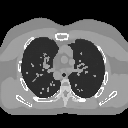
\includegraphics[width=\tempdima,height=\tempdima]{figures/experiments/xcat/blind_dps_axial.png}
                                        };
                                        \spy [yellow] on (0.05,-0.4) in node [left,yellow] at (1.2, 1.0);
                                \end{scope}
                        \end{tikzpicture}
                        \caption{\scriptsize JRM-ADM}
                \end{subfigure}
                \begin{subfigure}{0.19\linewidth}
                        \begin{tikzpicture}
                                \begin{scope}[spy using outlines={rounded rectangle, magnification=2, width=1.0cm, height=0.75cm, connect spies}]
                                        \node[inner sep=0pt] {
                                                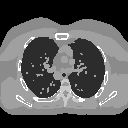
\includegraphics[width=\tempdima,height=\tempdima]{figures/experiments/xcat/gt_axial.png}
                                        };
                                        \spy [yellow] on (0.05,-0.4) in node [left,yellow] at (1.2, 1.0);
                                \end{scope}
                        \end{tikzpicture}
                        \caption{\scriptsize GT}
                \end{subfigure}

                \caption{
                        GT and end-inhale phase reconstructions on XCAT phantoms.
                }\label{fig:recon_xcat}

        \end{figure}

\end{frame}


\newlength{\reconimgsize}
\setlength{\reconimgsize}{0.17\linewidth}



\begin{frame}[fragile]
        \frametitle{Qualitative Evaluation of Reconstruction Methods}

        % %\newlength{\tempdima}
        % \setlength{\tempdima}{0.16\linewidth}



        % \only<1>{\begin{figure}
        %         \centering

        %         \begin{subfigure}{0.19\linewidth}
        %                 \begin{tikzpicture}
        %                         \begin{scope}[spy using outlines={rounded rectangle, magnification=2, width=1.0cm, height=0.75cm, connect spies}]
        %                                 \node[inner sep=0pt] {
        %                                         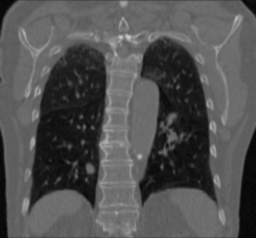
\includegraphics[width=\tempdima,height=\tempdima]{figures/experiments/recon_lung/gt_cor_0.png}
        %                                 };
        %                                 \spy [yellow] on (0.35,-0.3) in node [left,yellow] at (1.2, 1.0);
        %                         \end{scope}
        %                 \end{tikzpicture}
        %         \end{subfigure}
        %         \begin{subfigure}{0.19\linewidth}
        %                 \begin{tikzpicture}
        %                         \begin{scope}[spy using outlines={rounded rectangle, magnification=2, width=1.0cm, height=0.75cm, connect spies}]
        %                                 \node[inner sep=0pt] {
        %                                         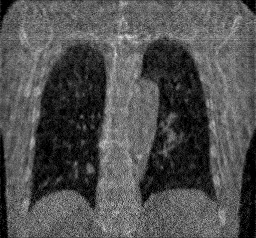
\includegraphics[width=\tempdima,height=\tempdima]{figures/experiments/recon_lung/fbp_cor_0.png}
        %                                 };
        %                                 \spy [yellow] on (0.35,-0.3) in node [left,yellow] at (1.2, 1.0);
        %                         \end{scope}
        %                 \end{tikzpicture}
        %         \end{subfigure}
        %         \begin{subfigure}{0.19\linewidth}
        %                 \begin{tikzpicture}
        %                         \begin{scope}[spy using outlines={rounded rectangle, magnification=2, width=1.0cm, height=0.75cm, connect spies}]
        %                                 \node[inner sep=0pt] {
        %                                         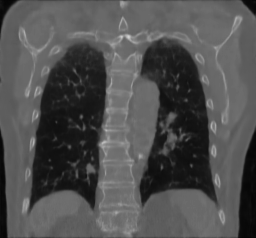
\includegraphics[width=\tempdima,height=\tempdima]{figures/experiments/recon_lung/gated_dps_cor_0.png}
        %                                 };
        %                                 \spy [yellow] on (0.35,-0.3) in node [left,yellow] at (1.2, 1.0);
        %                         \end{scope}
        %                 \end{tikzpicture}
        %         \end{subfigure}
        %         \begin{subfigure}{0.19\linewidth}
        %                 \begin{tikzpicture}
        %                         \begin{scope}[spy using outlines={rounded rectangle, magnification=2, width=1.0cm, height=0.75cm, connect spies}]
        %                                 \node[inner sep=0pt] {
        %                                         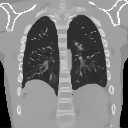
\includegraphics[width=\tempdima,height=\tempdima]{figures/experiments/xcat/blind_tv_coronal.png}
        %                                 };
        %                                 \spy [yellow] on (0.35,-0.3) in node [left,yellow] at (1.2, 1.0);
        %                         \end{scope}
        %                 \end{tikzpicture}
        %         \end{subfigure}
        %         \begin{subfigure}{0.19\linewidth}
        %                 \begin{tikzpicture}
        %                         \begin{scope}[spy using outlines={rounded rectangle, magnification=2, width=1.0cm, height=0.75cm, connect spies}]
        %                                 \node[inner sep=0pt] {
        %                                         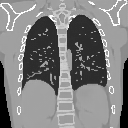
\includegraphics[width=\tempdima,height=\tempdima]{figures/experiments/xcat/blind_dps_coronal.png}
        %                                 };
        %                                 \spy [yellow] on (0.35,-0.3) in node [left,yellow] at (1.2, 1.0);
        %                         \end{scope}
        %                 \end{tikzpicture}
        %         \end{subfigure}


        %         \begin{subfigure}{0.19\linewidth}
        %                 \begin{tikzpicture}
        %                         \begin{scope}[spy using outlines={rounded rectangle, magnification=2, width=1.0cm, height=0.75cm, connect spies}]
        %                                 \node[inner sep=0pt] {
        %                                         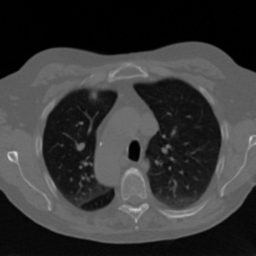
\includegraphics[width=\tempdima,height=\tempdima]{figures/experiments/recon_lung/gt_axe_0.png}
        %                                 };
        %                                 \spy [yellow] on (0.05,-0.4) in node [left,yellow] at (1.2, 1.0);
        %                         \end{scope}
        %                 \end{tikzpicture}
        %                 \caption{GT}
        %         \end{subfigure}
        %         \begin{subfigure}{0.19\linewidth}
        %                 \begin{tikzpicture}
        %                         \begin{scope}[spy using outlines={rounded rectangle, magnification=2, width=1.0cm, height=0.75cm, connect spies}]
        %                                 \node[inner sep=0pt] {
        %                                         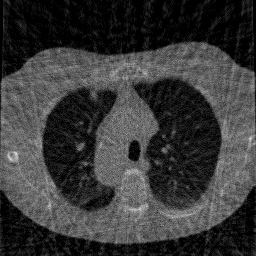
\includegraphics[width=\tempdima,height=\tempdima]{figures/experiments/recon_lung/fbp_axe_0.png}
        %                                 };
        %                                 \spy [yellow] on (0.05,-0.4) in node [left,yellow] at (1.2, 1.0);
        %                         \end{scope}
        %                 \end{tikzpicture}
        %                 \caption{Gated FBP}
        %         \end{subfigure}
        %         \begin{subfigure}{0.19\linewidth}
        %                 \begin{tikzpicture}
        %                         \begin{scope}[spy using outlines={rounded rectangle, magnification=2, width=1.0cm, height=0.75cm, connect spies}]
        %                                 \node[inner sep=0pt] {
        %                                         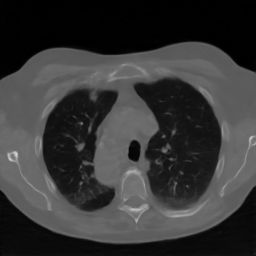
\includegraphics[width=\tempdima,height=\tempdima]{figures/experiments/recon_lung/gated_dps_axe_0.png}
        %                                 };
        %                                 \spy [yellow] on (0.05,-0.4) in node [left,yellow] at (1.2, 1.0);
        %                         \end{scope}
        %                 \end{tikzpicture}
        %                 \caption{Gated DPS}
        %         \end{subfigure}
        %         \begin{subfigure}{0.19\linewidth}
        %                 \begin{tikzpicture}
        %                         \begin{scope}[spy using outlines={rounded rectangle, magnification=2, width=1.0cm, height=0.75cm, connect spies}]
        %                                 \node[inner sep=0pt] {
        %                                         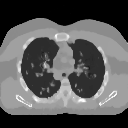
\includegraphics[width=\tempdima,height=\tempdima]{figures/experiments/xcat/blind_tv_axial.png}
        %                                 };
        %                                 \spy [yellow] on (0.05,-0.4) in node [left,yellow] at (1.2, 1.0);
        %                         \end{scope}
        %                 \end{tikzpicture}
        %                 \caption{JRM-TV}
        %         \end{subfigure}
        %         \begin{subfigure}{0.19\linewidth}
        %                 \begin{tikzpicture}
        %                         \begin{scope}[spy using outlines={rounded rectangle, magnification=2, width=1.0cm, height=0.75cm, connect spies}]
        %                                 \node[inner sep=0pt] {
        %                                         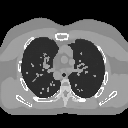
\includegraphics[width=\tempdima,height=\tempdima]{figures/experiments/xcat/blind_dps_axial.png}
        %                                 };
        %                                 \spy [yellow] on (0.05,-0.4) in node [left,yellow] at (1.2, 1.0);
        %                         \end{scope}
        %                 \end{tikzpicture}
        %                 \caption{JRM-ADM}
        %         \end{subfigure}

        %         \caption{
        %                 GT and end-inhale phase reconstructions on XCAT phantom.
        %         }
        % \end{figure}}


        %         \only<2>{\begin{figure}
        %         \centering

        %         \begin{subfigure}{0.19\linewidth}
        %                 \begin{tikzpicture}
        %                         \begin{scope}[spy using outlines={rounded rectangle, magnification=2, width=1.0cm, height=0.75cm, connect spies}]
        %                                 \node[inner sep=0pt] {
        %                                         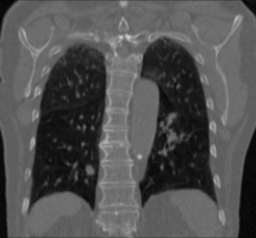
\includegraphics[width=\tempdima,height=\tempdima]{figures/experiments/recon_lung/gt_cor_1.png}
        %                                 };
        %                                 \spy [yellow] on (0.35,-0.3) in node [left,yellow] at (1.2, 1.0);
        %                         \end{scope}
        %                 \end{tikzpicture}
        %         \end{subfigure}
        %         \begin{subfigure}{0.19\linewidth}
        %                 \begin{tikzpicture}
        %                         \begin{scope}[spy using outlines={rounded rectangle, magnification=2, width=1.0cm, height=0.75cm, connect spies}]
        %                                 \node[inner sep=0pt] {
        %                                         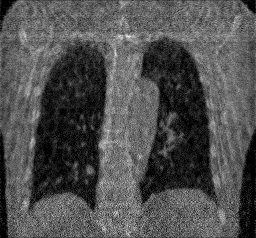
\includegraphics[width=\tempdima,height=\tempdima]{figures/experiments/recon_lung/fbp_cor_1.png}
        %                                 };
        %                                 \spy [yellow] on (0.35,-0.3) in node [left,yellow] at (1.2, 1.0);
        %                         \end{scope}
        %                 \end{tikzpicture}
        %         \end{subfigure}
        %         \begin{subfigure}{0.19\linewidth}
        %                 \begin{tikzpicture}
        %                         \begin{scope}[spy using outlines={rounded rectangle, magnification=2, width=1.0cm, height=0.75cm, connect spies}]
        %                                 \node[inner sep=0pt] {
        %                                         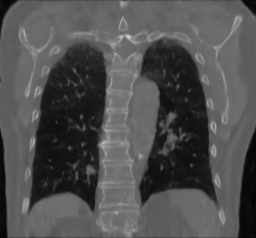
\includegraphics[width=\tempdima,height=\tempdima]{figures/experiments/recon_lung/gated_dps_cor_1.png}
        %                                 };
        %                                 \spy [yellow] on (0.35,-0.3) in node [left,yellow] at (1.2, 1.0);
        %                         \end{scope}
        %                 \end{tikzpicture}
        %         \end{subfigure}
        %         \begin{subfigure}{0.19\linewidth}
        %                 \begin{tikzpicture}
        %                         \begin{scope}[spy using outlines={rounded rectangle, magnification=2, width=1.0cm, height=0.75cm, connect spies}]
        %                                 \node[inner sep=0pt] {
        %                                         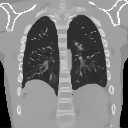
\includegraphics[width=\tempdima,height=\tempdima]{figures/experiments/xcat/blind_tv_coronal.png}
        %                                 };
        %                                 \spy [yellow] on (0.35,-0.3) in node [left,yellow] at (1.2, 1.0);
        %                         \end{scope}
        %                 \end{tikzpicture}
        %         \end{subfigure}
        %         \begin{subfigure}{0.19\linewidth}
        %                 \begin{tikzpicture}
        %                         \begin{scope}[spy using outlines={rounded rectangle, magnification=2, width=1.0cm, height=0.75cm, connect spies}]
        %                                 \node[inner sep=0pt] {
        %                                         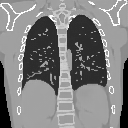
\includegraphics[width=\tempdima,height=\tempdima]{figures/experiments/xcat/blind_dps_coronal.png}
        %                                 };
        %                                 \spy [yellow] on (0.35,-0.3) in node [left,yellow] at (1.2, 1.0);
        %                         \end{scope}
        %                 \end{tikzpicture}
        %         \end{subfigure}


        %         \begin{subfigure}{0.19\linewidth}
        %                 \begin{tikzpicture}
        %                         \begin{scope}[spy using outlines={rounded rectangle, magnification=2, width=1.0cm, height=0.75cm, connect spies}]
        %                                 \node[inner sep=0pt] {
        %                                         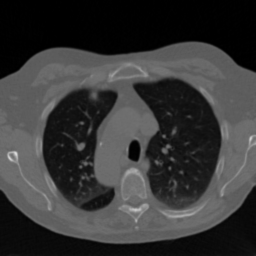
\includegraphics[width=\tempdima,height=\tempdima]{figures/experiments/recon_lung/gt_axe_1.png}
        %                                 };
        %                                 \spy [yellow] on (0.05,-0.4) in node [left,yellow] at (1.2, 1.0);
        %                         \end{scope}
        %                 \end{tikzpicture}
        %                 \caption{GT}
        %         \end{subfigure}
        %         \begin{subfigure}{0.19\linewidth}
        %                 \begin{tikzpicture}
        %                         \begin{scope}[spy using outlines={rounded rectangle, magnification=2, width=1.0cm, height=0.75cm, connect spies}]
        %                                 \node[inner sep=0pt] {
        %                                         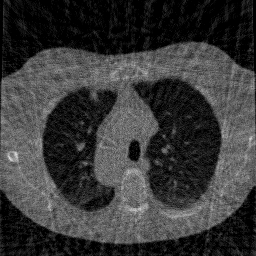
\includegraphics[width=\tempdima,height=\tempdima]{figures/experiments/recon_lung/fbp_axe_1.png}
        %                                 };
        %                                 \spy [yellow] on (0.05,-0.4) in node [left,yellow] at (1.2, 1.0);
        %                         \end{scope}
        %                 \end{tikzpicture}
        %                 \caption{Gated FBP}
        %         \end{subfigure}
        %         \begin{subfigure}{0.19\linewidth}
        %                 \begin{tikzpicture}
        %                         \begin{scope}[spy using outlines={rounded rectangle, magnification=2, width=1.0cm, height=0.75cm, connect spies}]
        %                                 \node[inner sep=0pt] {
        %                                         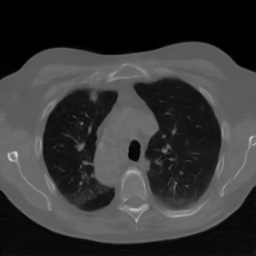
\includegraphics[width=\tempdima,height=\tempdima]{figures/experiments/recon_lung/gated_dps_axe_1.png}
        %                                 };
        %                                 \spy [yellow] on (0.05,-0.4) in node [left,yellow] at (1.2, 1.0);
        %                         \end{scope}
        %                 \end{tikzpicture}
        %                 \caption{Gated DPS}
        %         \end{subfigure}
        %         \begin{subfigure}{0.19\linewidth}
        %                 \begin{tikzpicture}
        %                         \begin{scope}[spy using outlines={rounded rectangle, magnification=2, width=1.0cm, height=0.75cm, connect spies}]
        %                                 \node[inner sep=0pt] {
        %                                         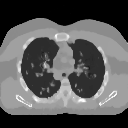
\includegraphics[width=\tempdima,height=\tempdima]{figures/experiments/xcat/blind_tv_axial.png}
        %                                 };
        %                                 \spy [yellow] on (0.05,-0.4) in node [left,yellow] at (1.2, 1.0);
        %                         \end{scope}
        %                 \end{tikzpicture}
        %                 \caption{JRM-TV}
        %         \end{subfigure}
        %         \begin{subfigure}{0.19\linewidth}
        %                 \begin{tikzpicture}
        %                         \begin{scope}[spy using outlines={rounded rectangle, magnification=2, width=1.0cm, height=0.75cm, connect spies}]
        %                                 \node[inner sep=0pt] {
        %                                         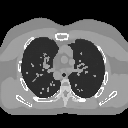
\includegraphics[width=\tempdima,height=\tempdima]{figures/experiments/xcat/blind_dps_axial.png}
        %                                 };
        %                                 \spy [yellow] on (0.05,-0.4) in node [left,yellow] at (1.2, 1.0);
        %                         \end{scope}
        %                 \end{tikzpicture}
        %                 \caption{JRM-ADM}
        %         \end{subfigure}

        %         \caption{
        %                 GT and end-inhale phase reconstructions on XCAT phantom.
        %         }
        % \end{figure}}


% use a fresh length name and make it slightly smaller

\newcommand{\ReconSubFig}[4][]{%
  \begin{subfigure}{\reconimgsize}
    \begin{tikzpicture}
      \begin{scope}[spy using outlines={
                        rounded rectangle,
                        magnification=2,
                        width=1.0cm,
                        height=0.75cm,
                        connect spies}]
        \node[inner sep=0pt]{%
          \includegraphics[width=\reconimgsize,height=\reconimgsize]{#2}%
        };
        \spy[yellow] on #3 in node[left,yellow] at #4;
      \end{scope}
    \end{tikzpicture}
    \ifx&#1&\else\caption{\scriptsize #1}\fi
  \end{subfigure}%
}


\only<1>{%
  \begin{figure}
    \centering
    % Coronal views (GT last)
    \makebox[\linewidth][c]{%
      \ReconSubFig{figures/experiments/recon_lung/fbp_cor_0.png}{(0.35,-0.6)}{(1.2,1.0)}\hfill
      \ReconSubFig{figures/experiments/recon_lung/gated_dps_cor_0.png}{(0.35,-0.6)}{(1.2,1.0)}\hfill
      \ReconSubFig{figures/experiments/recon_lung/jrm_tv_cor_0.png}{(0.35,-0.6)}{(1.2,1.0)}\hfill
      \ReconSubFig{figures/experiments/recon_lung/jrm_adm_cor_0.png}{(0.35,-0.6)}{(1.2,1.0)}\hfill
      \ReconSubFig{figures/experiments/recon_lung/gt_cor_0.png}{(0.35,-0.6)}{(1.2,1.0)}%
    }
    % Axial views (GT last)
    \makebox[\linewidth][c]{%
      \ReconSubFig[Gated FBP]{figures/experiments/recon_lung/fbp_axe_0.png}{(0.05,-0.4)}{(1.2,1.0)}\hfill
      \ReconSubFig[Gated DPS]{figures/experiments/recon_lung/gated_dps_axe_0.png}{(0.05,-0.4)}{(1.2,1.0)}\hfill
      \ReconSubFig[JRM-TV]{figures/experiments/recon_lung/jrm_tv_axe_0.png}{(0.05,-0.4)}{(1.2,1.0)}\hfill
      \ReconSubFig[JRM-ADM]{figures/experiments/recon_lung/jrm_adm_axe_0.png}{(0.05,-0.4)}{(1.2,1.0)}\hfill
      \ReconSubFig[GT]{figures/experiments/recon_lung/gt_axe_0.png}{(0.05,-0.4)}{(1.2,1.0)}%
    }
    \caption{GT and reconstructions on pseudo-real data.}
  \end{figure}%
}

\only<2>{%
  \begin{figure}
    \centering
    \makebox[\linewidth][c]{%
      \ReconSubFig{figures/experiments/recon_lung/fbp_cor_1.png}{(0.35,-0.6)}{(1.2,1.0)}\hfill
      \ReconSubFig{figures/experiments/recon_lung/gated_dps_cor_1.png}{(0.35,-0.6)}{(1.2,1.0)}\hfill
      \ReconSubFig{figures/experiments/recon_lung/jrm_tv_cor_1.png}{(0.35,-0.6)}{(1.2,1.0)}\hfill
      \ReconSubFig{figures/experiments/recon_lung/jrm_adm_cor_1.png}{(0.35,-0.6)}{(1.2,1.0)}\hfill
      \ReconSubFig{figures/experiments/recon_lung/gt_cor_1.png}{(0.35,-0.6)}{(1.2,1.0)}%
    }
    \makebox[\linewidth][c]{%
      \ReconSubFig[Gated FBP]{figures/experiments/recon_lung/fbp_axe_1.png}{(0.05,-0.4)}{(1.2,1.0)}\hfill
      \ReconSubFig[Gated DPS]{figures/experiments/recon_lung/gated_dps_axe_1.png}{(0.05,-0.4)}{(1.2,1.0)}\hfill
      \ReconSubFig[JRM-TV]{figures/experiments/recon_lung/jrm_tv_axe_1.png}{(0.05,-0.4)}{(1.2,1.0)}\hfill
      \ReconSubFig[JRM-ADM]{figures/experiments/recon_lung/jrm_adm_axe_1.png}{(0.05,-0.4)}{(1.2,1.0)}\hfill
      \ReconSubFig[GT]{figures/experiments/recon_lung/gt_axe_1.png}{(0.05,-0.4)}{(1.2,1.0)}%
    }
    \caption{GT and reconstructions on pseudo-real data.}
  \end{figure}%
}

\only<3>{%
  \begin{figure}
    \centering
    \makebox[\linewidth][c]{%
      \ReconSubFig{figures/experiments/recon_lung/fbp_cor_2.png}{(0.35,-0.6)}{(1.2,1.0)}\hfill
      \ReconSubFig{figures/experiments/recon_lung/gated_dps_cor_2.png}{(0.35,-0.6)}{(1.2,1.0)}\hfill
      \ReconSubFig{figures/experiments/recon_lung/jrm_tv_cor_2.png}{(0.35,-0.6)}{(1.2,1.0)}\hfill
      \ReconSubFig{figures/experiments/recon_lung/jrm_adm_cor_2.png}{(0.35,-0.6)}{(1.2,1.0)}\hfill
      \ReconSubFig{figures/experiments/recon_lung/gt_cor_2.png}{(0.35,-0.6)}{(1.2,1.0)}%
    }
    \makebox[\linewidth][c]{%
      \ReconSubFig[Gated FBP]{figures/experiments/recon_lung/fbp_axe_2.png}{(0.05,-0.4)}{(1.2,1.0)}\hfill
      \ReconSubFig[Gated DPS]{figures/experiments/recon_lung/gated_dps_axe_2.png}{(0.05,-0.4)}{(1.2,1.0)}\hfill
      \ReconSubFig[JRM-TV]{figures/experiments/recon_lung/jrm_tv_axe_2.png}{(0.05,-0.4)}{(1.2,1.0)}\hfill
      \ReconSubFig[JRM-ADM]{figures/experiments/recon_lung/jrm_adm_axe_2.png}{(0.05,-0.4)}{(1.2,1.0)}\hfill
      \ReconSubFig[GT]{figures/experiments/recon_lung/gt_axe_2.png}{(0.05,-0.4)}{(1.2,1.0)}%
    }
    \caption{GT and reconstructions on pseudo-real data.}
  \end{figure}%
}

\only<4>{%
  \begin{figure}
    \centering
    \makebox[\linewidth][c]{%
      \ReconSubFig{figures/experiments/recon_lung/fbp_cor_3.png}{(0.35,-0.6)}{(1.2,1.0)}\hfill
      \ReconSubFig{figures/experiments/recon_lung/gated_dps_cor_3.png}{(0.35,-0.6)}{(1.2,1.0)}\hfill
      \ReconSubFig{figures/experiments/recon_lung/jrm_tv_cor_3.png}{(0.35,-0.6)}{(1.2,1.0)}\hfill
      \ReconSubFig{figures/experiments/recon_lung/jrm_adm_cor_3.png}{(0.35,-0.6)}{(1.2,1.0)}\hfill
      \ReconSubFig{figures/experiments/recon_lung/gt_cor_3.png}{(0.35,-0.6)}{(1.2,1.0)}%
    }
    \makebox[\linewidth][c]{%
      \ReconSubFig[Gated FBP]{figures/experiments/recon_lung/fbp_axe_3.png}{(0.05,-0.4)}{(1.2,1.0)}\hfill
      \ReconSubFig[Gated DPS]{figures/experiments/recon_lung/gated_dps_axe_3.png}{(0.05,-0.4)}{(1.2,1.0)}\hfill
      \ReconSubFig[JRM-TV]{figures/experiments/recon_lung/jrm_tv_axe_3.png}{(0.05,-0.4)}{(1.2,1.0)}\hfill
      \ReconSubFig[JRM-ADM]{figures/experiments/recon_lung/jrm_adm_axe_3.png}{(0.05,-0.4)}{(1.2,1.0)}\hfill
      \ReconSubFig[GT]{figures/experiments/recon_lung/gt_axe_3.png}{(0.05,-0.4)}{(1.2,1.0)}%
    }
    \caption{GT and reconstructions on pseudo-real data.}
  \end{figure}%
}

\only<5>{%
  \begin{figure}
    \centering
    \makebox[\linewidth][c]{%
      \ReconSubFig{figures/experiments/recon_lung/fbp_cor_4.png}{(0.35,-0.6)}{(1.2,1.0)}\hfill
      \ReconSubFig{figures/experiments/recon_lung/gated_dps_cor_4.png}{(0.35,-0.6)}{(1.2,1.0)}\hfill
      \ReconSubFig{figures/experiments/recon_lung/jrm_tv_cor_4.png}{(0.35,-0.6)}{(1.2,1.0)}\hfill
      \ReconSubFig{figures/experiments/recon_lung/jrm_adm_cor_4.png}{(0.35,-0.6)}{(1.2,1.0)}\hfill
      \ReconSubFig{figures/experiments/recon_lung/gt_cor_4.png}{(0.35,-0.6)}{(1.2,1.0)}%
    }
    \makebox[\linewidth][c]{%
      \ReconSubFig[Gated FBP]{figures/experiments/recon_lung/fbp_axe_4.png}{(0.05,-0.4)}{(1.2,1.0)}\hfill
      \ReconSubFig[Gated DPS]{figures/experiments/recon_lung/gated_dps_axe_4.png}{(0.05,-0.4)}{(1.2,1.0)}\hfill
      \ReconSubFig[JRM-TV]{figures/experiments/recon_lung/jrm_tv_axe_4.png}{(0.05,-0.4)}{(1.2,1.0)}\hfill
      \ReconSubFig[JRM-ADM]{figures/experiments/recon_lung/jrm_adm_axe_4.png}{(0.05,-0.4)}{(1.2,1.0)}\hfill
      \ReconSubFig[GT]{figures/experiments/recon_lung/gt_axe_4.png}{(0.05,-0.4)}{(1.2,1.0)}%
    }
    \caption{GT and reconstructions on pseudo-real data.}
  \end{figure}%
}

\only<6>{%
  \begin{figure}
    \centering
    \makebox[\linewidth][c]{%
      \ReconSubFig{figures/experiments/recon_lung/fbp_cor_5.png}{(0.35,-0.6)}{(1.2,1.0)}\hfill
      \ReconSubFig{figures/experiments/recon_lung/gated_dps_cor_5.png}{(0.35,-0.6)}{(1.2,1.0)}\hfill
      \ReconSubFig{figures/experiments/recon_lung/jrm_tv_cor_5.png}{(0.35,-0.6)}{(1.2,1.0)}\hfill
      \ReconSubFig{figures/experiments/recon_lung/jrm_adm_cor_5.png}{(0.35,-0.6)}{(1.2,1.0)}\hfill
      \ReconSubFig{figures/experiments/recon_lung/gt_cor_5.png}{(0.35,-0.6)}{(1.2,1.0)}%
    }
    \makebox[\linewidth][c]{%
      \ReconSubFig[Gated FBP]{figures/experiments/recon_lung/fbp_axe_5.png}{(0.05,-0.4)}{(1.2,1.0)}\hfill
      \ReconSubFig[Gated DPS]{figures/experiments/recon_lung/gated_dps_axe_5.png}{(0.05,-0.4)}{(1.2,1.0)}\hfill
      \ReconSubFig[JRM-TV]{figures/experiments/recon_lung/jrm_tv_axe_5.png}{(0.05,-0.4)}{(1.2,1.0)}\hfill
      \ReconSubFig[JRM-ADM]{figures/experiments/recon_lung/jrm_adm_axe_5.png}{(0.05,-0.4)}{(1.2,1.0)}\hfill
      \ReconSubFig[GT]{figures/experiments/recon_lung/gt_axe_5.png}{(0.05,-0.4)}{(1.2,1.0)}%
    }
    \caption{GT and reconstructions on pseudo-real data.}
  \end{figure}%
}

\only<7>{%
  \begin{figure}
    \centering
    \makebox[\linewidth][c]{%
      \ReconSubFig{figures/experiments/recon_lung/fbp_cor_6.png}{(0.35,-0.6)}{(1.2,1.0)}\hfill
      \ReconSubFig{figures/experiments/recon_lung/gated_dps_cor_6.png}{(0.35,-0.6)}{(1.2,1.0)}\hfill
      \ReconSubFig{figures/experiments/recon_lung/jrm_tv_cor_6.png}{(0.35,-0.6)}{(1.2,1.0)}\hfill
      \ReconSubFig{figures/experiments/recon_lung/jrm_adm_cor_6.png}{(0.35,-0.6)}{(1.2,1.0)}\hfill
      \ReconSubFig{figures/experiments/recon_lung/gt_cor_6.png}{(0.35,-0.6)}{(1.2,1.0)}%
    }
    \makebox[\linewidth][c]{%
      \ReconSubFig[Gated FBP]{figures/experiments/recon_lung/fbp_axe_6.png}{(0.05,-0.4)}{(1.2,1.0)}\hfill
      \ReconSubFig[Gated DPS]{figures/experiments/recon_lung/gated_dps_axe_6.png}{(0.05,-0.4)}{(1.2,1.0)}\hfill
      \ReconSubFig[JRM-TV]{figures/experiments/recon_lung/jrm_tv_axe_6.png}{(0.05,-0.4)}{(1.2,1.0)}\hfill
      \ReconSubFig[JRM-ADM]{figures/experiments/recon_lung/jrm_adm_axe_6.png}{(0.05,-0.4)}{(1.2,1.0)}\hfill
      \ReconSubFig[GT]{figures/experiments/recon_lung/gt_axe_6.png}{(0.05,-0.4)}{(1.2,1.0)}%
    }
    \caption{GT and reconstructions on pseudo-real data.}
  \end{figure}%
}

\only<8>{%
  \begin{figure}
    \centering
    \makebox[\linewidth][c]{%
      \ReconSubFig{figures/experiments/recon_lung/fbp_cor_7.png}{(0.35,-0.6)}{(1.2,1.0)}\hfill
      \ReconSubFig{figures/experiments/recon_lung/gated_dps_cor_7.png}{(0.35,-0.6)}{(1.2,1.0)}\hfill
      \ReconSubFig{figures/experiments/recon_lung/jrm_tv_cor_7.png}{(0.35,-0.6)}{(1.2,1.0)}\hfill
      \ReconSubFig{figures/experiments/recon_lung/jrm_adm_cor_7.png}{(0.35,-0.6)}{(1.2,1.0)}\hfill
      \ReconSubFig{figures/experiments/recon_lung/gt_cor_7.png}{(0.35,-0.6)}{(1.2,1.0)}%
    }
    \makebox[\linewidth][c]{%
      \ReconSubFig[Gated FBP]{figures/experiments/recon_lung/fbp_axe_7.png}{(0.05,-0.4)}{(1.2,1.0)}\hfill
      \ReconSubFig[Gated DPS]{figures/experiments/recon_lung/gated_dps_axe_7.png}{(0.05,-0.4)}{(1.2,1.0)}\hfill
      \ReconSubFig[JRM-TV]{figures/experiments/recon_lung/jrm_tv_axe_7.png}{(0.05,-0.4)}{(1.2,1.0)}\hfill
      \ReconSubFig[JRM-ADM]{figures/experiments/recon_lung/jrm_adm_axe_7.png}{(0.05,-0.4)}{(1.2,1.0)}\hfill
      \ReconSubFig[GT]{figures/experiments/recon_lung/gt_axe_7.png}{(0.05,-0.4)}{(1.2,1.0)}%
    }
    \caption{GT and reconstructions on pseudo-real data.}
  \end{figure}%
}

\only<9>{%
  \begin{figure}
    \centering
    \makebox[\linewidth][c]{%
      \ReconSubFig{figures/experiments/recon_lung/fbp_cor_8.png}{(0.35,-0.6)}{(1.2,1.0)}\hfill
      \ReconSubFig{figures/experiments/recon_lung/gated_dps_cor_8.png}{(0.35,-0.6)}{(1.2,1.0)}\hfill
      \ReconSubFig{figures/experiments/recon_lung/jrm_tv_cor_8.png}{(0.35,-0.6)}{(1.2,1.0)}\hfill
      \ReconSubFig{figures/experiments/recon_lung/jrm_adm_cor_8.png}{(0.35,-0.6)}{(1.2,1.0)}\hfill
      \ReconSubFig{figures/experiments/recon_lung/gt_cor_8.png}{(0.35,-0.6)}{(1.2,1.0)}%
    }
    \makebox[\linewidth][c]{%
      \ReconSubFig[Gated FBP]{figures/experiments/recon_lung/fbp_axe_8.png}{(0.05,-0.4)}{(1.2,1.0)}\hfill
      \ReconSubFig[Gated DPS]{figures/experiments/recon_lung/gated_dps_axe_8.png}{(0.05,-0.4)}{(1.2,1.0)}\hfill
      \ReconSubFig[JRM-TV]{figures/experiments/recon_lung/jrm_tv_axe_8.png}{(0.05,-0.4)}{(1.2,1.0)}\hfill
      \ReconSubFig[JRM-ADM]{figures/experiments/recon_lung/jrm_adm_axe_8.png}{(0.05,-0.4)}{(1.2,1.0)}\hfill
      \ReconSubFig[GT]{figures/experiments/recon_lung/gt_axe_8.png}{(0.05,-0.4)}{(1.2,1.0)}%
    }
    \caption{GT and reconstructions on pseudo-real data.}
  \end{figure}%
}

\only<10>{%
  \begin{figure}
    \centering
    \makebox[\linewidth][c]{%
      \ReconSubFig{figures/experiments/recon_lung/fbp_cor_9.png}{(0.35,-0.6)}{(1.2,1.0)}\hfill
      \ReconSubFig{figures/experiments/recon_lung/gated_dps_cor_9.png}{(0.35,-0.6)}{(1.2,1.0)}\hfill
      \ReconSubFig{figures/experiments/recon_lung/jrm_tv_cor_9.png}{(0.35,-0.6)}{(1.2,1.0)}\hfill
      \ReconSubFig{figures/experiments/recon_lung/jrm_adm_cor_9.png}{(0.35,-0.6)}{(1.2,1.0)}\hfill
      \ReconSubFig{figures/experiments/recon_lung/gt_cor_9.png}{(0.35,-0.6)}{(1.2,1.0)}%
    }
    \makebox[\linewidth][c]{%
      \ReconSubFig[Gated FBP]{figures/experiments/recon_lung/fbp_axe_9.png}{(0.05,-0.4)}{(1.2,1.0)}\hfill
      \ReconSubFig[Gated DPS]{figures/experiments/recon_lung/gated_dps_axe_9.png}{(0.05,-0.4)}{(1.2,1.0)}\hfill
      \ReconSubFig[JRM-TV]{figures/experiments/recon_lung/jrm_tv_axe_9.png}{(0.05,-0.4)}{(1.2,1.0)}\hfill
      \ReconSubFig[JRM-ADM]{figures/experiments/recon_lung/jrm_adm_axe_9.png}{(0.05,-0.4)}{(1.2,1.0)}\hfill
      \ReconSubFig[GT]{figures/experiments/recon_lung/gt_axe_9.png}{(0.05,-0.4)}{(1.2,1.0)}%
    }
    \caption{GT and reconstructions on pseudo-real data.}
  \end{figure}%
}


%   \only<1>{%
%     \begin{figure}
%       \centering
%       \makebox[\linewidth][c]{%
%         \ReconSubFig{figures/experiments/recon_lung/gt_cor_0.png}{(0.35,-0.6)}{(1.2,1.0)}\hfill
%         \ReconSubFig{figures/experiments/recon_lung/fbp_cor_0.png}{(0.35,-0.6)}{(1.2,1.0)}\hfill
%         \ReconSubFig{figures/experiments/recon_lung/gated_dps_cor_0.png}{(0.35,-0.6)}{(1.2,1.0)}\hfill
%         \ReconSubFig{figures/experiments/recon_lung/jrm_tv_cor_0.png}{(0.35,-0.6)}{(1.2,1.0)}\hfill
%         \ReconSubFig{figures/experiments/recon_lung/jrm_adm_cor_0.png}{(0.35,-0.6)}{(1.2,1.0)}%
%       }

%       \makebox[\linewidth][c]{%
%         \ReconSubFig[GT]{figures/experiments/recon_lung/gt_axe_0.png}{(0.05,-0.4)}{(1.2,1.0)}\hfill
%         \ReconSubFig[Gated FBP]{figures/experiments/recon_lung/fbp_axe_0.png}{(0.05,-0.4)}{(1.2,1.0)}\hfill
%         \ReconSubFig[Gated DPS]{figures/experiments/recon_lung/gated_dps_axe_0.png}{(0.05,-0.4)}{(1.2,1.0)}\hfill
%         \ReconSubFig[JRM-TV]{figures/experiments/recon_lung/jrm_tv_axe_0.png}{(0.05,-0.4)}{(1.2,1.0)}\hfill
%         \ReconSubFig[JRM-ADM]{figures/experiments/recon_lung/jrm_adm_axe_0.png}{(0.05,-0.4)}{(1.2,1.0)}%
%       }
%       \caption{GT and reconstructions on pseudo-real data.}
%     \end{figure}%
%   }

%   \only<2>{%
%     \begin{figure}
%       \centering
%       \makebox[\linewidth][c]{%
%         \ReconSubFig{figures/experiments/recon_lung/gt_cor_1.png}{(0.35,-0.6)}{(1.2,1.0)}\hfill
%         \ReconSubFig{figures/experiments/recon_lung/fbp_cor_1.png}{(0.35,-0.6)}{(1.2,1.0)}\hfill
%         \ReconSubFig{figures/experiments/recon_lung/gated_dps_cor_1.png}{(0.35,-0.6)}{(1.2,1.0)}\hfill
%         \ReconSubFig{figures/experiments/recon_lung/jrm_tv_cor_1.png}{(0.35,-0.6)}{(1.2,1.0)}\hfill
%         \ReconSubFig{figures/experiments/recon_lung/jrm_adm_cor_1.png}{(0.35,-0.6)}{(1.2,1.0)}%
%       }

%       \makebox[\linewidth][c]{%
%         \ReconSubFig[GT]{figures/experiments/recon_lung/gt_axe_1.png}{(0.05,-0.4)}{(1.2,1.0)}\hfill
%         \ReconSubFig[Gated FBP]{figures/experiments/recon_lung/fbp_axe_1.png}{(0.05,-0.4)}{(1.2,1.0)}\hfill
%         \ReconSubFig[Gated DPS]{figures/experiments/recon_lung/gated_dps_axe_1.png}{(0.05,-0.4)}{(1.2,1.0)}\hfill
%         \ReconSubFig[JRM-TV]{figures/experiments/recon_lung/jrm_tv_axe_1.png}{(0.05,-0.4)}{(1.2,1.0)}\hfill
%         \ReconSubFig[JRM-ADM]{figures/experiments/recon_lung/jrm_adm_axe_1.png}{(0.05,-0.4)}{(1.2,1.0)}%
%       }
%       \caption{GT and reconstructions on pseudo-real data.}
%     \end{figure}%
%   }

%     \only<3>{%
%     \begin{figure}
%       \centering
%       \makebox[\linewidth][c]{%
%         \ReconSubFig{figures/experiments/recon_lung/gt_cor_2.png}{(0.35,-0.6)}{(1.2,1.0)}\hfill
%         \ReconSubFig{figures/experiments/recon_lung/fbp_cor_2.png}{(0.35,-0.6)}{(1.2,1.0)}\hfill
%         \ReconSubFig{figures/experiments/recon_lung/gated_dps_cor_2.png}{(0.35,-0.6)}{(1.2,1.0)}\hfill
%         \ReconSubFig{figures/experiments/recon_lung/jrm_tv_cor_2.png}{(0.35,-0.6)}{(1.2,1.0)}\hfill
%         \ReconSubFig{figures/experiments/recon_lung/jrm_adm_cor_2.png}{(0.35,-0.6)}{(1.2,1.0)}%
%       }

%       \makebox[\linewidth][c]{%
%         \ReconSubFig[GT]{figures/experiments/recon_lung/gt_axe_2.png}{(0.05,-0.4)}{(1.2,1.0)}\hfill
%         \ReconSubFig[Gated FBP]{figures/experiments/recon_lung/fbp_axe_2.png}{(0.05,-0.4)}{(1.2,1.0)}\hfill
%         \ReconSubFig[Gated DPS]{figures/experiments/recon_lung/gated_dps_axe_2.png}{(0.05,-0.4)}{(1.2,1.0)}\hfill
%         \ReconSubFig[JRM-TV]{figures/experiments/recon_lung/jrm_tv_axe_2.png}{(0.05,-0.4)}{(1.2,1.0)}\hfill
%         \ReconSubFig[JRM-ADM]{figures/experiments/recon_lung/jrm_adm_axe_2.png}{(0.05,-0.4)}{(1.2,1.0)}%
%       }
%       \caption{GT and reconstructions on pseudo-real data.}
%     \end{figure}%
%   }

%   \only<4>{%
%     \begin{figure}
%       \centering
%       \makebox[\linewidth][c]{%
%         \ReconSubFig{figures/experiments/recon_lung/gt_cor_3.png}{(0.35,-0.6)}{(1.2,1.0)}\hfill
%         \ReconSubFig{figures/experiments/recon_lung/fbp_cor_3.png}{(0.35,-0.6)}{(1.2,1.0)}\hfill
%         \ReconSubFig{figures/experiments/recon_lung/gated_dps_cor_3.png}{(0.35,-0.6)}{(1.2,1.0)}\hfill
%         \ReconSubFig{figures/experiments/recon_lung/jrm_tv_cor_3.png}{(0.35,-0.6)}{(1.2,1.0)}\hfill
%         \ReconSubFig{figures/experiments/recon_lung/jrm_adm_cor_3.png}{(0.35,-0.6)}{(1.2,1.0)}%
%       }

%       \makebox[\linewidth][c]{%
%         \ReconSubFig[GT]{figures/experiments/recon_lung/gt_axe_3.png}{(0.05,-0.4)}{(1.2,1.0)}\hfill
%         \ReconSubFig[Gated FBP]{figures/experiments/recon_lung/fbp_axe_3.png}{(0.05,-0.4)}{(1.2,1.0)}\hfill
%         \ReconSubFig[Gated DPS]{figures/experiments/recon_lung/gated_dps_axe_3.png}{(0.05,-0.4)}{(1.2,1.0)}\hfill
%         \ReconSubFig[JRM-TV]{figures/experiments/recon_lung/jrm_tv_axe_3.png}{(0.05,-0.4)}{(1.2,1.0)}\hfill
%         \ReconSubFig[JRM-ADM]{figures/experiments/recon_lung/jrm_adm_axe_3.png}{(0.05,-0.4)}{(1.2,1.0)}%
%       }
%       \caption{GT and reconstructions on pseudo-real data.}
%     \end{figure}%
%   }

%   \only<5>{%
%     \begin{figure}
%       \centering
%       \makebox[\linewidth][c]{%
%         \ReconSubFig{figures/experiments/recon_lung/gt_cor_4.png}{(0.35,-0.6)}{(1.2,1.0)}\hfill
%         \ReconSubFig{figures/experiments/recon_lung/fbp_cor_4.png}{(0.35,-0.6)}{(1.2,1.0)}\hfill
%         \ReconSubFig{figures/experiments/recon_lung/gated_dps_cor_4.png}{(0.35,-0.6)}{(1.2,1.0)}\hfill
%         \ReconSubFig{figures/experiments/recon_lung/jrm_tv_cor_4.png}{(0.35,-0.6)}{(1.2,1.0)}\hfill
%         \ReconSubFig{figures/experiments/recon_lung/jrm_adm_cor_4.png}{(0.35,-0.6)}{(1.2,1.0)}%
%       }

%       \makebox[\linewidth][c]{%
%         \ReconSubFig[GT]{figures/experiments/recon_lung/gt_axe_4.png}{(0.05,-0.4)}{(1.2,1.0)}\hfill
%         \ReconSubFig[Gated FBP]{figures/experiments/recon_lung/fbp_axe_4.png}{(0.05,-0.4)}{(1.2,1.0)}\hfill
%         \ReconSubFig[Gated DPS]{figures/experiments/recon_lung/gated_dps_axe_4.png}{(0.05,-0.4)}{(1.2,1.0)}\hfill
%         \ReconSubFig[JRM-TV]{figures/experiments/recon_lung/jrm_tv_axe_4.png}{(0.05,-0.4)}{(1.2,1.0)}\hfill
%         \ReconSubFig[JRM-ADM]{figures/experiments/recon_lung/jrm_adm_axe_4.png}{(0.05,-0.4)}{(1.2,1.0)}%
%       }
%       \caption{GT and reconstructions on pseudo-real data.}
%     \end{figure}%
%   }


%   \only<6>{%
%     \begin{figure}
%       \centering
%       \makebox[\linewidth][c]{%
%         \ReconSubFig{figures/experiments/recon_lung/gt_cor_5.png}{(0.35,-0.6)}{(1.2,1.0)}\hfill
%         \ReconSubFig{figures/experiments/recon_lung/fbp_cor_5.png}{(0.35,-0.6)}{(1.2,1.0)}\hfill
%         \ReconSubFig{figures/experiments/recon_lung/gated_dps_cor_5.png}{(0.35,-0.6)}{(1.2,1.0)}\hfill
%         \ReconSubFig{figures/experiments/recon_lung/jrm_tv_cor_5.png}{(0.35,-0.6)}{(1.2,1.0)}\hfill
%         \ReconSubFig{figures/experiments/recon_lung/jrm_adm_cor_5.png}{(0.35,-0.6)}{(1.2,1.0)}%
%       }

%       \makebox[\linewidth][c]{%
%         \ReconSubFig[GT]{figures/experiments/recon_lung/gt_axe_5.png}{(0.05,-0.4)}{(1.2,1.0)}\hfill
%         \ReconSubFig[Gated FBP]{figures/experiments/recon_lung/fbp_axe_5.png}{(0.05,-0.4)}{(1.2,1.0)}\hfill
%         \ReconSubFig[Gated DPS]{figures/experiments/recon_lung/gated_dps_axe_5.png}{(0.05,-0.4)}{(1.2,1.0)}\hfill
%         \ReconSubFig[JRM-TV]{figures/experiments/recon_lung/jrm_tv_axe_5.png}{(0.05,-0.4)}{(1.2,1.0)}\hfill
%         \ReconSubFig[JRM-ADM]{figures/experiments/recon_lung/jrm_adm_axe_5.png}{(0.05,-0.4)}{(1.2,1.0)}%
%       }
%       \caption{GT and reconstructions on pseudo-real data.}
%     \end{figure}%
%   }

%   \only<7>{%
%     \begin{figure}
%       \centering
%       \makebox[\linewidth][c]{%
%         \ReconSubFig{figures/experiments/recon_lung/gt_cor_6.png}{(0.35,-0.6)}{(1.2,1.0)}\hfill
%         \ReconSubFig{figures/experiments/recon_lung/fbp_cor_6.png}{(0.35,-0.6)}{(1.2,1.0)}\hfill
%         \ReconSubFig{figures/experiments/recon_lung/gated_dps_cor_6.png}{(0.35,-0.6)}{(1.2,1.0)}\hfill
%         \ReconSubFig{figures/experiments/recon_lung/jrm_tv_cor_6.png}{(0.35,-0.6)}{(1.2,1.0)}\hfill
%         \ReconSubFig{figures/experiments/recon_lung/jrm_adm_cor_6.png}{(0.35,-0.6)}{(1.2,1.0)}%
%       }

%       \makebox[\linewidth][c]{%
%         \ReconSubFig[GT]{figures/experiments/recon_lung/gt_axe_6.png}{(0.05,-0.4)}{(1.2,1.0)}\hfill
%         \ReconSubFig[Gated FBP]{figures/experiments/recon_lung/fbp_axe_6.png}{(0.05,-0.4)}{(1.2,1.0)}\hfill
%         \ReconSubFig[Gated DPS]{figures/experiments/recon_lung/gated_dps_axe_6.png}{(0.05,-0.4)}{(1.2,1.0)}\hfill
%         \ReconSubFig[JRM-TV]{figures/experiments/recon_lung/jrm_tv_axe_6.png}{(0.05,-0.4)}{(1.2,1.0)}\hfill
%         \ReconSubFig[JRM-ADM]{figures/experiments/recon_lung/jrm_adm_axe_6.png}{(0.05,-0.4)}{(1.2,1.0)}%
%       }
%       \caption{GT and reconstructions on pseudo-real data.}
%     \end{figure}%
%   }

%   \only<8>{%
%     \begin{figure}
%       \centering
%       \makebox[\linewidth][c]{%
%         \ReconSubFig{figures/experiments/recon_lung/gt_cor_7.png}{(0.35,-0.6)}{(1.2,1.0)}\hfill
%         \ReconSubFig{figures/experiments/recon_lung/fbp_cor_7.png}{(0.35,-0.6)}{(1.2,1.0)}\hfill
%         \ReconSubFig{figures/experiments/recon_lung/gated_dps_cor_7.png}{(0.35,-0.6)}{(1.2,1.0)}\hfill
%         \ReconSubFig{figures/experiments/recon_lung/jrm_tv_cor_7.png}{(0.35,-0.6)}{(1.2,1.0)}\hfill
%         \ReconSubFig{figures/experiments/recon_lung/jrm_adm_cor_7.png}{(0.35,-0.6)}{(1.2,1.0)}%
%       }

%       \makebox[\linewidth][c]{%
%         \ReconSubFig[GT]{figures/experiments/recon_lung/gt_axe_7.png}{(0.05,-0.4)}{(1.2,1.0)}\hfill
%         \ReconSubFig[Gated FBP]{figures/experiments/recon_lung/fbp_axe_7.png}{(0.05,-0.4)}{(1.2,1.0)}\hfill
%         \ReconSubFig[Gated DPS]{figures/experiments/recon_lung/gated_dps_axe_7.png}{(0.05,-0.4)}{(1.2,1.0)}\hfill
%         \ReconSubFig[JRM-TV]{figures/experiments/recon_lung/jrm_tv_axe_7.png}{(0.05,-0.4)}{(1.2,1.0)}\hfill
%         \ReconSubFig[JRM-ADM]{figures/experiments/recon_lung/jrm_adm_axe_7.png}{(0.05,-0.4)}{(1.2,1.0)}%
%       }
%       \caption{GT and reconstructions on pseudo-real data.}
%     \end{figure}%
%   }

%     \only<9>{%
%     \begin{figure}
%       \centering
%       \makebox[\linewidth][c]{%
%         \ReconSubFig{figures/experiments/recon_lung/gt_cor_8.png}{(0.35,-0.6)}{(1.2,1.0)}\hfill
%         \ReconSubFig{figures/experiments/recon_lung/fbp_cor_8.png}{(0.35,-0.6)}{(1.2,1.0)}\hfill
%         \ReconSubFig{figures/experiments/recon_lung/gated_dps_cor_8.png}{(0.35,-0.6)}{(1.2,1.0)}\hfill
%         \ReconSubFig{figures/experiments/recon_lung/jrm_tv_cor_8.png}{(0.35,-0.6)}{(1.2,1.0)}\hfill
%         \ReconSubFig{figures/experiments/recon_lung/jrm_adm_cor_8.png}{(0.35,-0.6)}{(1.2,1.0)}%
%       }

%       \makebox[\linewidth][c]{%
%         \ReconSubFig[GT]{figures/experiments/recon_lung/gt_axe_8.png}{(0.05,-0.4)}{(1.2,1.0)}\hfill
%         \ReconSubFig[Gated FBP]{figures/experiments/recon_lung/fbp_axe_8.png}{(0.05,-0.4)}{(1.2,1.0)}\hfill
%         \ReconSubFig[Gated DPS]{figures/experiments/recon_lung/gated_dps_axe_8.png}{(0.05,-0.4)}{(1.2,1.0)}\hfill
%         \ReconSubFig[JRM-TV]{figures/experiments/recon_lung/jrm_tv_axe_8.png}{(0.05,-0.4)}{(1.2,1.0)}\hfill
%         \ReconSubFig[JRM-ADM]{figures/experiments/recon_lung/jrm_adm_axe_8.png}{(0.05,-0.4)}{(1.2,1.0)}%
%       }
%       \caption{GT and reconstructions on pseudo-real data.}
%     \end{figure}%
%   }


%     \only<10>{%
%     \begin{figure}
%       \centering
%       \makebox[\linewidth][c]{%
%         \ReconSubFig{figures/experiments/recon_lung/gt_cor_9.png}{(0.35,-0.6)}{(1.2,1.0)}\hfill
%         \ReconSubFig{figures/experiments/recon_lung/fbp_cor_9.png}{(0.35,-0.6)}{(1.2,1.0)}\hfill
%         \ReconSubFig{figures/experiments/recon_lung/gated_dps_cor_9.png}{(0.35,-0.6)}{(1.2,1.0)}\hfill
%         \ReconSubFig{figures/experiments/recon_lung/jrm_tv_cor_9.png}{(0.35,-0.6)}{(1.2,1.0)}\hfill
%         \ReconSubFig{figures/experiments/recon_lung/jrm_adm_cor_9.png}{(0.35,-0.6)}{(1.2,1.0)}%
%       }

%       \makebox[\linewidth][c]{%
%         \ReconSubFig[GT]{figures/experiments/recon_lung/gt_axe_9.png}{(0.05,-0.4)}{(1.2,1.0)}\hfill
%         \ReconSubFig[Gated FBP]{figures/experiments/recon_lung/fbp_axe_9.png}{(0.05,-0.4)}{(1.2,1.0)}\hfill
%         \ReconSubFig[Gated DPS]{figures/experiments/recon_lung/gated_dps_axe_9.png}{(0.05,-0.4)}{(1.2,1.0)}\hfill
%         \ReconSubFig[JRM-TV]{figures/experiments/recon_lung/jrm_tv_axe_9.png}{(0.05,-0.4)}{(1.2,1.0)}\hfill
%         \ReconSubFig[JRM-ADM]{figures/experiments/recon_lung/jrm_adm_axe_9.png}{(0.05,-0.4)}{(1.2,1.0)}%
%       }
%       \caption{GT and reconstructions on pseudo-real data.}
%     \end{figure}%
%   }


\end{frame}


\begin{frame}[fragile]
        \frametitle{Extension to Motion-Corrected Sparse-View Head CBCT \cite{de2025adaptive}: Quantitative Results}

        \begin{table}[t]
                \scriptsize
                \centering
                \begin{tabular}{lcccccc}
                        \toprule
                        Views & Method  & PSNR $(\uparrow)$          & SSIM $(\uparrow)$         & MAE $\tau$ $(\downarrow)$ & MAE $\vartheta$ $(\downarrow)$ \\
                        \midrule
                        \multirow{3}{*}{60}
                              & FDK     & 17.00                      & 0.23                      & -                         & -                              \\
                              & JRM-TV  & 28.91                      & 0.90                      & 0.34                      & 0.11                           \\
                              & JRM-ADM & \underline{\textbf{29.67}} & \underline{\textbf{0.92}} & \underline{\textbf{0.27}} & \underline{\textbf{0.09}}      \\
                        \midrule
                        \multirow{3}{*}{40}
                              & FDK     & 16.92                      & 0.19                      & -                         & -                              \\
                              & JRM-TV  & 27.19                      & 0.87                      & 0.43                      & 0.12                           \\
                              & JRM-ADM & \underline{\textbf{28.66}} & \underline{\textbf{0.91}} & \underline{\textbf{0.29}} & \underline{\textbf{0.11}}      \\
                        \midrule
                        \multirow{3}{*}{20}
                              & FDK     & 14.96                      & 0.14                      & -                         & -                              \\
                              & JRM-TV  & 23.38                      & 0.75                      & 0.86                      & 0.17                           \\
                              & JRM-ADM & \underline{\textbf{27.18}} & \underline{\textbf{0.87}} & \underline{\textbf{0.30}} & \underline{\textbf{0.12}}      \\
                        \bottomrule
                \end{tabular}
                \caption{Quantitative results of methods in comparison on the CQ500 \cite{chilamkurthy2018deep} dataset for the motion corrected reconstruction tasks under sparse-view settings of 60, 40, and 20 views.}
        \end{table}
\end{frame}




\begin{frame}[fragile]
        \frametitle{Extension to Motion-Corrected Sparse-View Head CBCT \cite{de2025adaptive}: Qualitative Results}

        % \newlength{\tempdima}
        \setlength{\tempdima}{0.19\linewidth}

        \begin{figure}

                \noindent
                \begin{minipage}[c]{0.01\linewidth}
                        \centering
                        \rotatebox{90}{\footnotesize 60 views }
                \end{minipage}%
                \begin{minipage}[c]{0.99\linewidth}
                        \centering
                        \begin{subfigure}{0.22\linewidth}
                                \begin{tikzpicture}
                                        \begin{scope}[spy using outlines={rounded rectangle, magnification=2, width=1.0cm, height=0.75cm, connect spies}]
                                                \node[inner sep=0pt] {
                                                        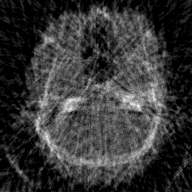
\includegraphics[width=\tempdima,height=\tempdima]{figures/experiments/recon_head/fdk40_slice_d.png}
                                                };
                                                \spy [yellow] on (0.45,-0.10) in node [left,yellow] at (1.2, 1.0);
                                        \end{scope}
                                \end{tikzpicture}
                        \end{subfigure}
                        \begin{subfigure}{0.22\linewidth}
                                \begin{tikzpicture}
                                        \begin{scope}[spy using outlines={rounded rectangle, magnification=2, width=1.0cm, height=0.75cm, connect spies}]
                                                \node[inner sep=0pt] {
                                                        \includegraphics[width=\tempdima,height=\tempdima]{figures/experiments/recon_head/jrmtv40_slice_d.png}
                                                };
                                                \spy [yellow] on (0.45,-0.10) in node [left,yellow] at (1.2, 1.0);
                                        \end{scope}
                                \end{tikzpicture}
                        \end{subfigure}
                        \begin{subfigure}{0.22\linewidth}
                                \begin{tikzpicture}
                                        \begin{scope}[spy using outlines={rounded rectangle, magnification=2, width=1.0cm, height=0.75cm, connect spies}]
                                                \node[inner sep=0pt] {
                                                        \includegraphics[width=\tempdima,height=\tempdima]{figures/experiments/recon_head/jrmadm40_slice_d.png}
                                                };
                                                \spy [yellow] on (0.45,-0.10) in node [left,yellow] at (1.2, 1.0);
                                        \end{scope}
                                \end{tikzpicture}
                        \end{subfigure}
                        \begin{subfigure}{0.22\linewidth}
                                \begin{tikzpicture}
                                        \begin{scope}[spy using outlines={rounded rectangle, magnification=2, width=1.0cm, height=0.75cm, connect spies}]
                                                \node[inner sep=0pt] {
                                                        \includegraphics[width=\tempdima,height=\tempdima]{./figures/experiments/recon_head/gt_slice_d.png}
                                                };
                                                \spy [yellow] on (0.45,-0.10) in node [left,yellow] at (1.2, 1.0);
                                        \end{scope}
                                \end{tikzpicture}
                        \end{subfigure}
                \end{minipage}

                \noindent
                \begin{minipage}[c]{0.01\linewidth}
                        \centering
                        \rotatebox{90}{\footnotesize 20 views }
                \end{minipage}%
                \begin{minipage}[c]{0.99\linewidth}
                        \centering
                        \begin{subfigure}{0.22\linewidth}
                                \begin{tikzpicture}
                                        \begin{scope}[spy using outlines={rounded rectangle, magnification=2, width=1.0cm, height=0.75cm, connect spies}]
                                                \node[inner sep=0pt] {
                                                        \includegraphics[width=\tempdima,height=\tempdima]{figures/experiments/recon_head/fdk20_slice_d.png}
                                                };
                                                \spy [yellow] on (0.45,-0.10) in node [left,yellow] at (1.2, 1.0);
                                        \end{scope}
                                \end{tikzpicture}
                                \caption{FDK}
                        \end{subfigure}
                        \begin{subfigure}{0.22\linewidth}
                                \begin{tikzpicture}
                                        \begin{scope}[spy using outlines={rounded rectangle, magnification=2, width=1.0cm, height=0.75cm, connect spies}]
                                                \node[inner sep=0pt] {
                                                        \includegraphics[width=\tempdima,height=\tempdima]{figures/experiments/recon_head/jrmtv20_slice_d.png}
                                                };
                                                \spy [yellow] on (0.45,-0.10) in node [left,yellow] at (1.2, 1.0);
                                        \end{scope}
                                \end{tikzpicture}
                                \caption{JRM-TV}
                        \end{subfigure}
                        \begin{subfigure}{0.22\linewidth}
                                \begin{tikzpicture}
                                        \begin{scope}[spy using outlines={rounded rectangle, magnification=2, width=1.0cm, height=0.75cm, connect spies}]
                                                \node[inner sep=0pt] {
                                                        \includegraphics[width=\tempdima,height=\tempdima]{figures/experiments/recon_head/jrmadm20_slice_d.png}
                                                };
                                                \spy [yellow] on (0.45,-0.10) in node [left,yellow] at (1.2, 1.0);
                                        \end{scope}
                                \end{tikzpicture}
                                \caption{JRM-ADM}
                        \end{subfigure}
                        \begin{subfigure}{0.22\linewidth}
                                \begin{tikzpicture}
                                        \begin{scope}[spy using outlines={rounded rectangle, magnification=2, width=1.0cm, height=0.75cm, connect spies}]
                                                \node[inner sep=0pt] {
                                                        \includegraphics[width=\tempdima,height=\tempdima]{figures/experiments/recon_head/gt_slice_d.png}
                                                };
                                                \spy [yellow] on (0.45,-0.10) in node [left,yellow] at (1.2, 1.0);
                                        \end{scope}
                                \end{tikzpicture}
                                \caption{GT}
                        \end{subfigure}
                \end{minipage}

                \caption{GT and reconstructions (axial plane) for motion-affected sparse-view CBCT: results are shown for 40- and 20-view acquisition settings.}
        \end{figure}

\end{frame}
  \section{Conclusion - Discussion}


\begin{frame}[fragile]
  \frametitle{Conclusion \& Discussion}

  \begin{itemize}
    \item<1-> \textbf{High-fidelity 4DCT:} JRM-ADM yields artifact-free, high-resolution reconstructions under irregular breathing, outperforming classical reconstruction methods.
    \item<2-> \textbf{Computational Challenges:} GPU memory and runtime remain high; future work should explore how to solve this.
    \item<3-> \textbf{Real World Challenges:} Working on real sinograms would be the best path toward clinical translation.
  \end{itemize}
\end{frame}
  \begin{frame}{Acknowledgments}

    \vfill

    This work was supported the French \textbf{National Institute of Health and Medical Research (Inserm)}, by the \textbf{University of Western Brittany (UBO)}, by \textbf{France Life Imaging} under grant No ANR-11-INBS-0006 and by \textbf{CPER 2021–2027 IMAGIIS
(INNOV-XS)}.

    \vfill

    \begin{figure}
        \includegraphics[width=0.8\textwidth]{figures/cover/logo.png}
    \end{figure}

    \vfill
    
\end{frame}

%   \appendix
%   \input{content/appendix.tex}


  % \begin{frame}[allowframebreaks]{References}
  %   \bibliography{biblio/references}
  % \end{frame}


  \begin{frame}[allowframebreaks]{References}
    \printbibliography[heading=none]
  \end{frame}

\end{document}